\documentclass[12pt,a4paper,openany]{book}

% ===== PACKAGES =====
\usepackage[utf8]{inputenc}
\usepackage[T1]{fontenc}
\usepackage{microtype}
\usepackage{amsmath,amssymb,amsthm}
\usepackage{graphicx}
\usepackage{xcolor}
\usepackage{tikz}
\usepackage{listings}
\usepackage{hyperref}
\usepackage{booktabs}
\usepackage{enumitem}
\usepackage{fancyhdr}
\usepackage{titlesec}
\usepackage{tcolorbox}
\usepackage{fontawesome5}
\usepackage{mdframed}
\usepackage{subcaption}
\usepackage{wrapfig}
\usepackage{gensymb}
\usepackage{pgfplots}
\pgfplotsset{width=10cm,compat=1.9}
\usepackage{amsmath}
\usetikzlibrary{shapes.geometric, arrows}


% speech bubbles - will become useful for protocols with 2 participants
\newcommand{\speechleft}[2]{%
    \begin{tcolorbox}[colback=blue!10, colframe=blue!50, arc=3mm, left=2mm, right=2mm, boxrule=1pt, before skip=5mm, after skip=5mm]
        \textbf{#1:} #2
    \end{tcolorbox}
}

\newcommand{\speechright}[2]{%
    \begin{tcolorbox}[colback=green!10, colframe=green!50, arc=3mm, left=2mm, right=2mm, boxrule=1pt, before skip=5mm, after skip=5mm, halign=right]
        \textbf{#1:} #2
    \end{tcolorbox}
}

% ===== GEOMETRY - SMALLER MARGINS =====
\usepackage[
    top=3cm,
    bottom=3cm,
    left=3cm,
    right=3cm,
    marginparwidth=1.8cm,
    marginparsep=0.3cm,
    headheight=15pt,
    headsep=1cm,
    footskip=1cm
]{geometry}

% ===== COLORS =====
\definecolor{noteblue}{RGB}{13, 110, 253}
\definecolor{tipgreen}{RGB}{25, 135, 84}
\definecolor{importantorange}{RGB}{255, 149, 0}
\definecolor{warningyellow}{RGB}{255, 193, 7}
\definecolor{cautionred}{RGB}{220, 53, 69}
\definecolor{codegray}{RGB}{248, 249, 250}
\definecolor{linkblue}{RGB}{0, 123, 255}

% ===== HYPERREF SETUP =====
\hypersetup{
    colorlinks=true,
    linkcolor=linkblue,
    citecolor=linkblue,
    urlcolor=linkblue,
    bookmarksdepth=3,
    pdfborder={0 0 0}
}

% ===== GITHUB-STYLE CALLOUT BOXES =====
\tcbuselibrary{skins,breakable}

% Base style for all callouts - GitHub-like design
\tcbset{
    calloutbase/.style={
        enhanced,
        breakable,
        sharp corners,
        colback=white,
        colframe=#1,
        borderline west={3pt}{0pt}{#1},
        boxrule=1pt,
        left=12pt,
        right=8pt,
        top=8pt,
        bottom=8pt,
        fonttitle=\bfseries\sffamily\small,
        coltitle=#1,
        title style={left color=#1!10, right color=#1!5},
        before skip=1.5\baselineskip,
        after skip=1.5\baselineskip,
    }
}

% NOTE callout - Blue theme
\newtcolorbox{noteblock}{
    calloutbase=noteblue,
    colback=noteblue!3,
    title={\textcolor{noteblue}{\faInfoCircle}\ \textcolor{noteblue}{NOTE}}
}

% TIP callout - Green theme  
\newtcolorbox{tipblock}{
    calloutbase=tipgreen,
    colback=tipgreen!3,
    title={\textcolor{tipgreen}{\faLightbulb}\ \textcolor{tipgreen}{TIP}}
}

% IMPORTANT callout - Orange theme
\newtcolorbox{importantblock}{
    calloutbase=importantorange,
    colback=importantorange!3,
    title={\textcolor{importantorange}{\faExclamationCircle}\ \textcolor{importantorange}{IMPORTANT}}
}

% WARNING callout - Yellow theme
\newtcolorbox{warningblock}{
    calloutbase=warningyellow,
    colback=warningyellow!3,
    title={\textcolor{warningyellow!80!black}{\faExclamationTriangle}\ \textcolor{warningyellow!80!black}{WARNING}}
}

% CAUTION callout - Red theme
\newtcolorbox{cautionblock}{
    calloutbase=cautionred,
    colback=cautionred!3,
    title={\textcolor{cautionred}{\faExclamationTriangle}\ \textcolor{cautionred}{CAUTION}}
}
% ===== CODE LISTINGS - C LANGUAGE =====
\lstset{
    backgroundcolor=\color{codegray},
    basicstyle=\ttfamily\footnotesize,
    breakatwhitespace=false,
    breaklines=true,
    captionpos=b,
    commentstyle=\color{gray},
    frame=single,
    frameround=tttt,
    framesep=5pt,
    keywordstyle=\color{blue},
    language=C,
    numbers=left,
    numbersep=5pt,
    numberstyle=\tiny\color{gray},
    rulecolor=\color{black},
    showspaces=false,
    showstringspaces=false,
    showtabs=false,
    stringstyle=\color{red},
    tabsize=4,
    morekeywords={size_t, ssize_t, socklen_t, struct, typedef}
}

% ===== CHAPTER AND SECTION FORMATTING =====
\titleformat{\chapter}[display]
  {\normalfont\huge\bfseries\sffamily}
  {\chaptertitlename\ \thechapter}
  {20pt}
  {\Huge}
  
\titleformat{\section}
  {\normalfont\Large\bfseries\sffamily}
  {\thesection}
  {1em}
  {}
  
\titleformat{\subsection}
  {\normalfont\large\bfseries\sffamily}
  {\thesubsection}
  {1em}
  {}

% ===== HEADER AND FOOTER =====
\pagestyle{fancy}
\fancyhf{}
\fancyhead[LE]{\small\sffamily\color{darkblue}\nouppercase{\leftmark}}
\fancyhead[RO]{\small\sffamily\color{darkblue}\nouppercase{\rightmark}}
\fancyfoot[C]{\small\sffamily\color{darkblue}\thepage}
\renewcommand{\headrulewidth}{0.5pt}
\renewcommand{\headrule}{\hbox to\headwidth{\color{darkblue!30}\leaders\hrule height \headrulewidth\hfill}}
\renewcommand{\footrulewidth}{0pt}

\fancypagestyle{plain}{
    \fancyhf{}
    \fancyfoot[C]{\small\sffamily\color{darkblue}\thepage}
    \renewcommand{\headrulewidth}{0pt}
    \renewcommand{\footrulewidth}{0pt}
}

% ===== THEOREM ENVIRONMENTS =====
\theoremstyle{definition}
\newtheorem{definition}{Definition}[chapter]
\newtheorem{example}{Example}[chapter]
\newtheorem{protocol}{Protocol}[chapter]

\theoremstyle{plain}
\newtheorem{theorem}{Theorem}[chapter]
\newtheorem{lemma}{Lemma}[chapter]

% ===== DOCUMENT METADATA =====
\title{Computer Networks: Course Reader}
\author{Computer Networks TAs et al.}
\date{Latest revision: \today}


% ===== FONT SETUP =====
\usepackage{charter} % Charter for main text
\usepackage[expert]{mathdesign} % Matching math fonts for Charter
\usepackage[scaled=0.9]{helvet} % Helvetica for sans-serif
\usepackage[scaled=0.85]{FiraMono} % Fira Code for monospace
\renewcommand{\sfdefault}{phv} % Ensure Helvetica is used for sans-serif


% ===== OTHER =====
\setlength{\parindent}{0pt}
\setlength{\parskip}{0.5\baselineskip}
\setcounter{tocdepth}{1}
% link color dark blue
\definecolor{darkblue}{RGB}{0, 51, 102}
\hypersetup{
    linkcolor=darkblue,
    citecolor=darkblue,
    urlcolor=darkblue
}

\newcommand{\version}{v0.1.30}
 % Include version command
% Version stamp using draftwatermark
\usepackage[firstpageonly=true]{draftwatermark}
\SetWatermarkText{\sffamily\bfseries\version!}
\SetWatermarkScale{0.5}
\SetWatermarkAngle{-30}
\SetWatermarkHorCenter{0.8\paperwidth}
\SetWatermarkVerCenter{0.11\paperheight}
\SetWatermarkLightness{0.85}
\SetWatermarkColor{darkblue!10!white}


\begin{document}

% ===== TITLE PAGE =====
\frontmatter
\begin{titlepage}
    \vspace*{\fill}
    \centering
    {\fontsize{40}{48}\selectfont\bfseries\sffamily Computer Networks}\\[0.5cm]
    {\fontsize{30}{36}\selectfont\sffamily Course Reader}

    \vspace{1.5cm}

    \begin{tikzpicture}
        \draw[thick, darkblue] (0,0) -- (14,0);
        \fill[darkblue] (7,0) circle (3pt);
    \end{tikzpicture}

    \vspace{2cm}

    {\fontsize{20}{24}\selectfont\sffamily Computer Networks TAs et al.}

    \vspace*{\fill}

    % Bottom section with date and version
    \centering

    {\fontsize{16}{19}\selectfont\sffamily\textbf{Latest Revision:} \today}\\[0.3cm]
    \vspace{0.5cm}
    
\includegraphics[width=0.5\textwidth]{assets/rug.png}

    \vspace{1cm}
    
\end{titlepage}

\newpage
\thispagestyle{empty}
\mbox{}
% ===== TABLE OF CONTENTS =====
\tableofcontents

% Clear headers for preface
\markboth{}{}
\chapter{Preface}
\section*{Welcome to the CN Reader}
This reader was inspired by the wonderfully crafted Languages \& Machines reader - a course you will all take during your second year as a Computing Science student (at the time of writing this).

What follows is the \textbf{first edition} of this reader, so please be patient with us if we have made any mistakes and/or omissions.

The first edition was developed by Boyan Karakostov and Mihai David in 2025.

\begin{warningblock}
This reader should not be considered a replacement for lecture slides and tutorials. We strongly encourage you to attend all sessions provided by the course.
\end{warningblock}

\section*{How to Use This Reader}
This reader is designed to be a companion to the course, providing additional explanations, examples, and exercises. It is structured to follow the course syllabus, with each section corresponding to a topic covered in lectures.

\section*{Prerequisites}
This reader assumes basic familiarity with C programming and various computer science concepts. If you are new to C or need a refresher, consider reviewing introductory materials on C programming.

\section*{Feedback}
We welcome your feedback on this reader. If you find any errors, have suggestions for improvements, or would like to see additional topics covered, please reach out to the professor of this course or visit the reader's \href{https://github.com/Code-For-Groningen/CN-Reader}{GitHub repository}\footnote{For the paper readers: github.com/Code-For-Groningen/CN-Reader}.

\section*{License and Usage}
This reader is licensed under the \href{https://creativecommons.org/licenses/by-nc-sa/4.0/}{Creative Commons Attribution-NonCommercial-ShareAlike 4.0 International License}. You are free to share and adapt the material for non-commercial purposes, provided you give appropriate credit, indicate if changes were made, and distribute your contributions under the same license.

The code exerpts are licensed under GNU General Public License v3.0.

\section*{Updates and Errata}
This reader is a living document. We will periodically update it to correct errors, add new content, and improve clarity. Please check the \href{https://github.com/Code-For-Groningen/CN-Reader}{GitHub repository} for the latest version and any errata. The PDF provided by the course is a snapshot of the reader at the time of publication, and may not include the latest changes (but it will always be the most stable version).

If you'd like to report an error or suggest an improvement, please open an issue or submit a pull request on the GitHub repository. We appreciate your contributions to making this reader better for everyone.

% ===== MAIN CONTENT =====
\mainmatter
% ---- Setup and Introduction ----
\chapter{Introduction}
\section{Overview}
Computer Networks is a course that covers the fundamental concepts and technologies that enable communication between computers and devices. 

Understanding how data flows through networks, the protocols that govern this communication, and the architecture of network systems is not only essential for understanding modern computing but could also be pretty fun!

This course will explore various topics including:
\begin{itemize}
    \item The OSI and TCP/IP models
    \item Network protocols and standards
    \item IP addressing and subnetting
    \item Routing and switching
    \item Wireless networking
    \item Network security
\end{itemize}

For the practical component, we will be using Wireshark and Cisco Packet Tracer to analyze network traffic and simulate network configurations. There will be sections dedicated to guides as to how to set up and use these tools effectively.

Your practical assignments will involve programming in C \textbf{on Linux} to implement network protocols and other miscellaneous tasks.

\begin{importantblock}
Networking is handled differently depending on the operating system and C does not attempt to abstract this away. We implore you to check out why that is in detail, but for the purposes of this reader, this will be the only mention of it. The mandatory \textit{Operating Systems} course will cover some of the differences in more detail.

From here on out, we will assume you are using Linux or an equivalent Unix-like operating system. If you are using Windows, you will need to familiarize yourself with the \href{https://docs.microsoft.com/en-us/windows/wsl/install}{Windows Subsystem for Linux (WSL)} or use a virtual machine with a Linux distribution installed.
\end{importantblock}

\section{Setting Up Your Environment}

There are multiple tools and libraries that you will need to install to complete the practical assignments in this course. Follow the instructions below to set up your environment.

\subsection{Windows}
As mentioned earlier, for code, you will need to use the Windows Subsystem for Linux (WSL) or a virtual machine with a Linux distribution installed.

As for the tools, please download and install the following:
\begin{itemize}
    \item \href{https://www.wireshark.org/download.html}{Wireshark}
    \item \href{https://www.netacad.com/cisco-packet-tracer}{Cisco Packet Tracer}
\end{itemize}

\subsection{Linux}

\subsubsection{Debian-based systems (Ubuntu, Debian, Linux Mint)}\label{sec:debian-install}
For Debian-based distributions, you can install Wireshark using the package manager:
\begin{verbatim}
sudo apt update
sudo apt install wireshark
\end{verbatim}

\begin{noteblock}
Cisco Packet Tracer is not available in official repositories. Download it from the \href{https://www.netacad.com/courses/packet-tracer}{Cisco Networking Academy} website and follow their installation instructions.
\end{noteblock}

\subsubsection{Arch-based systems}
For Arch-based distributions:
\begin{verbatim}
sudo pacman -S wireshark-qt
\end{verbatim}

Cisco Packet Tracer can be installed from the AUR\@:
\begin{verbatim}
yay -S packettracer
\end{verbatim}

\subsection{macOS}
For macOS, you can install Wireshark using Homebrew:
\begin{verbatim}
brew install --cask wireshark
\end{verbatim}

Cisco Packet Tracer can be downloaded from the \href{https://www.netacad.com/courses/packet-tracer}{Cisco Networking Academy} website. While macOS is Unix-like, the C networking libraries should work \textbf{similarly to Linux}, though there may be minor differences in some system calls and headers.

\section{C Development Environment}

In addition to the networking tools above, you'll need a proper C development environment for the programming assignments.

\subsection{Essential Development Tools}

All systems will need:
\begin{itemize}
    \item A C compiler (GCC usually)
    \item Make build system
    \item A text editor or IDE
\end{itemize}

\subsubsection{Linux Installation}

On Debian-based systems:
\begin{verbatim}
sudo apt install build-essential git
\end{verbatim}

On Arch-based systems:
\begin{verbatim}
sudo pacman -S base-devel git
\end{verbatim}

\subsubsection{macOS Installation}

Install Xcode Command Line Tools:
\begin{verbatim}
xcode-select --install
\end{verbatim}

\subsection{Networking Libraries}

The assignments will use standard POSIX networking libraries that are included with your system:
\begin{itemize}
    \item \texttt{sys/socket.h} - Socket programming interface
    \item \texttt{netinet/in.h} - Internet address family
    \item \texttt{arpa/inet.h} - Internet operations
    \item \texttt{unistd.h} - POSIX operating system API
\end{itemize}

\begin{noteblock}
These are part of the standard C library on Unix-like systems.
\end{noteblock}
\chapter{The OSI Model}\label{sec:osi_intro}
\section{What is OSI?}
\begin{figure}[h]
    \centering
    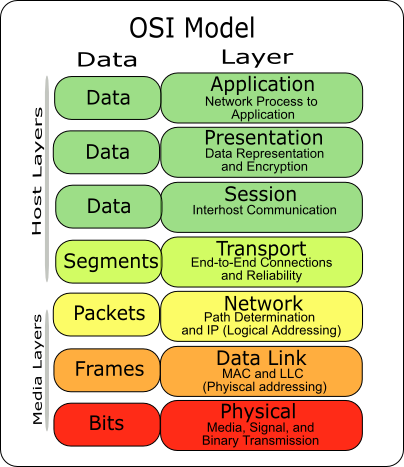
\includegraphics[width=.6\textwidth]{assets/osi/layers.png}
    \caption{The OSI Model Layers}\label{fig:osi_layers_intro}
\end{figure}
From chaos to order, the Open Systems Interconnection (OSI) model is a framework we use to understand how different networking protocols interact. Coincidentally (not so much), the Computer Networks course is structured around it.

You don't need to memorize these layers right off the bat, as, instead of that, we would like for you to understand each layer's purpose \textit{before} knowing the correct term for it. That way, you will be able to come up with the term yourself!

\section{Why OSI? $\star$}
The development of the model began in the late 1970s as a collaborative effort to standardize networking (See Figure \ref{fig:standards}). The model emerged from the need to connect networking systems that were using proprietary protocols from vendors like IBM and DEC.

\vspace{1em}
\begin{figure}[h]
    \centering
    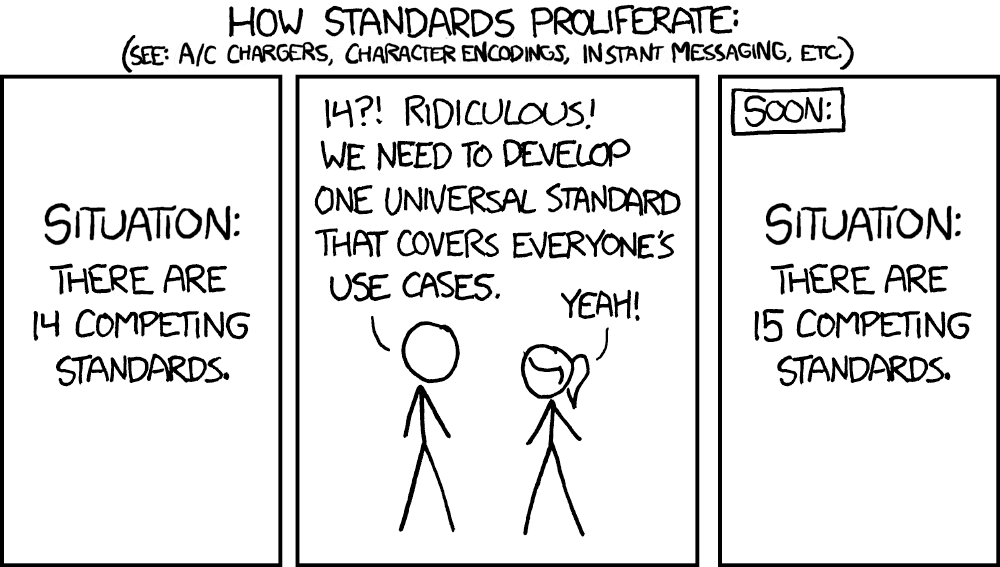
\includegraphics[width=.6\textwidth]{assets/osi/physical/standards.png}
    \caption{XKCD \#927: \href{https://xkcd.com/927/}{Standards}}
    \label{fig:standards}
\end{figure}

The OSI model was formally defined in 1978 by Hubert Zimmermann and published as an ISO\footnote{
    You're going to be seeing this acronym a lot, so let's get it out of the way: ISO stands for International Organization for Standardization.
} standard in 1984. Despite its comprehensive framework, it ultimately lost to the simpler TCP/IP model (Figure \ref{fig:osi_vs_tcpip}), which during the `Protocol Wars' of the 1980s and 1990s. Nonetheless, the OSI model remains a valuable tool for understanding networking concepts and protocols.

\begin{figure}[h]
    \centering
    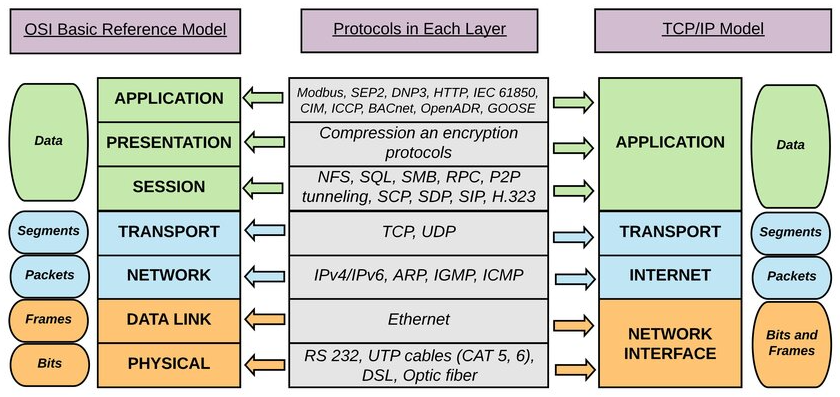
\includegraphics[width=.7\textwidth]{assets/osi/physical/tcp_vs_osi.png}
    \caption{OSI vs TCP/IP}
    \label{fig:osi_vs_tcpip}
\end{figure}








% Physical Layer
\chapter{Physical Layer}\label{sec:osi_physical}
\section{tl;dr}
The first layer of the OSI model is responsible for the physical transmission of data over a medium, with little to no concern for the content involved. It defines the hardware elements used in the communication process, such as cables, switches, and network interface cards (NICs).

\begin{noteblock}
    It might come across as a surprise, but routers are \textbf{not} part of the Physical Layer. The intuition as to why that is is that routers \textit{route}, hence they need to understand the content of the packets they are forwarding. This is a function of the Network Layer (Layer 3) in the OSI model.
\end{noteblock}

The Physical Layer is responsible for:
\begin{itemize}
    \item Converting bits to electrical, optical, or radio signals
    \item Defining voltage levels, timing, and physical data rates
    \item Specifying physical connectors and cable types
    \item Managing the physical topology of the network (which we'll be using Cisco Packet Tracer to visualize)
    \item Synchronizing transmission between devices
\end{itemize}

\newpage

% mediums
\section{Transmission Media}\label{sec:transmission_media}
Different physical media carry the signals that transport our data across networks:

\subsection*{Guided Media}
Guided media confines signals to a specific path (literally "guided" along a cable or fiber). 

\subsubsection*{Twisted Pair Cable}
You probably know this one well, as you find it in most local area networks (LANs) and telephone systems. It consists of pairs of insulated copper wires twisted together to reduce electromagnetic interference.

\begin{figure}[h]
    \centering
    
\includegraphics[width=4cm]{assets/osi/physical/f-utp.png}
    \caption{F-UTP}\label{fig:twisted_pair}
\end{figure}

UTP (Unshielded Twisted Pair) is the most common type, but there are also shielded variants like STP (Shielded Twisted Pair) and F/UTP (Foiled Unshielded Twisted Pair).

\vspace{1em}

\subsubsection*{Coaxial Cable}
Usually used in cable television and broadband\footnote{Everything but dial-up.}.

\begin{figure}[h]
    \centering
    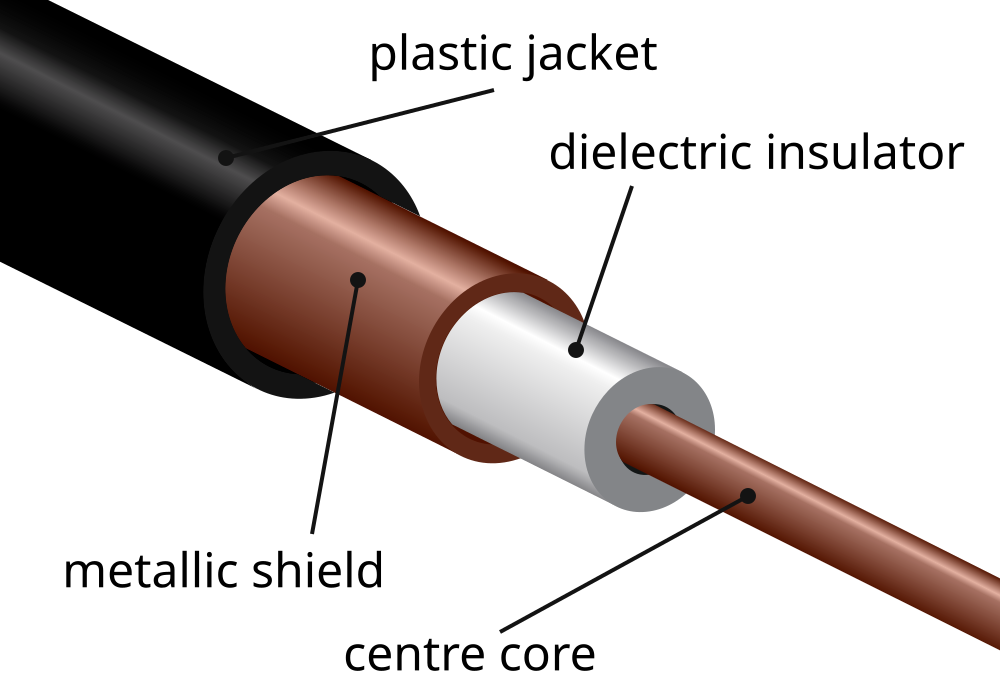
\includegraphics[width=4cm]{assets/osi/physical/coax.png}
    \caption{Coaxial cable structure}\label{fig:coaxial_cable}
\end{figure}

\begin{itemize}
    \item Common in cable TV networks and was used in early Ethernet implementations
    \item Offers better noise immunity than twisted pair with higher bandwidth capacity, which is why radio amateurs still use it
\end{itemize}

\vspace{1em}

\newpage
\subsubsection*{Fiber Optic Cable}
Uses light to transmit data, making it the fastest and most reliable medium available today.

\begin{itemize}
    \item Composed of a core, cladding, and protective outer layer
    \item Immune to electromagnetic interference
    \item Supports high bandwidths
\end{itemize}

\begin{figure}
    \centering
    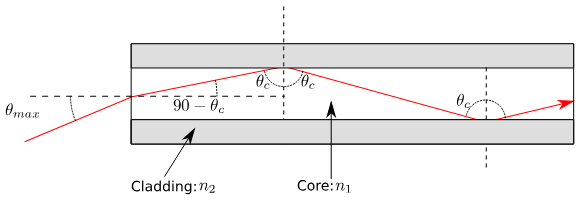
\includegraphics[width=.8\textwidth]{assets/osi/physical/fiber.png}
    \caption{Fiber optic cable structure}\label{fig:fiber_optic}
\end{figure}

\vspace{1em}

\subsection*{Wireless Transmission}
Ever wondered how signals travel through the air? Different types of electromagnetic waves are used for wireless communication, each with its own characteristics.

% assets/osi/physical/spectrum.png
\begin{figure}[h]
    \centering
    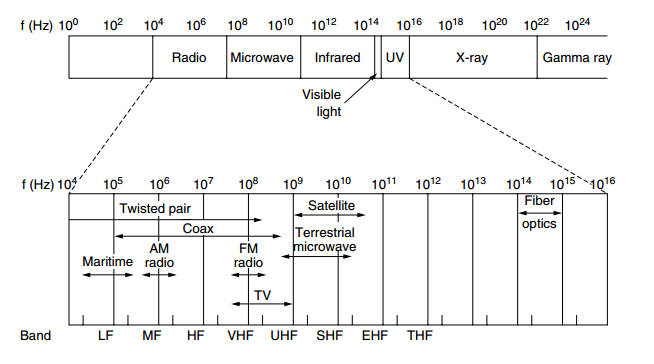
\includegraphics[width=.8\textwidth]{assets/osi/physical/spectrum.png}
    \caption{Electromagnetic spectrum showing different types of waves}\label{fig:em_spectrum}
\end{figure}

\subsubsection*{Radio Waves}
Radio waves are used for various wireless communication systems, including Wi-Fi, Bluetooth, and cellular networks. They can travel long distances (depending on wavelength) and penetrate through obstacles like walls.

\begin{noteblock}
    Fun fact! A lot of appliances like car remotes, thermostats and RC toys operate on the 433 MHz frequency band, which is a part of the radio spectrum. This is a perfect entry point if you'd like to hack your own devices or learn about radio communication.
\end{noteblock}

\subsubsection*{Microwaves}
Contrary to popular belief, microwaves are not just for cooking food. They are also used for point-to-point communication links, satellite communications, and some Wi-Fi networks. Microwaves have shorter wavelengths than radio waves, allowing them to carry more data, but faster attenuation\footnote{
    Attenuation: Reduction in signal strength as it travels through a medium, which can be caused by absorption, scattering, or reflection. 
    This is why we need repeaters/amplifiers!
} over distance.

\section{Standards and Specifications}
\subsection*{Ethernet Standards}
\begin{table}[h]
    \centering
    \begin{tabular}{|c|c|c|c|}
        \hline
        \textbf{Standard} & \textbf{Speed} & \textbf{Media} & \textbf{Distance} \\
        \hline
        10BASE-T & 10 Mbps & Cat3 UTP & 100m \\
        100BASE-TX & 100 Mbps & Cat5 UTP & 100m \\
        1000BASE-T & 1 Gbps & Cat5e UTP & 100m \\
        10GBASE-T & 10 Gbps & Cat6a UTP & 100m \\
        1000BASE-SX & 1 Gbps & Multi-mode fiber & 550m \\
        \hline
    \end{tabular}
    \caption{Common Ethernet Physical Layer Standards}\label{tab:ethernet_standards}
\end{table}

\subsection*{WiFi Standards}
\begin{itemize}
    \item 802.11a: 5 GHz, up to 54 Mbps
    \item 802.11b: 2.4 GHz, up to 11 Mbps
    \item 802.11g: 2.4 GHz, up to 54 Mbps
    \item 802.11n: 2.4/5 GHz, up to 600 Mbps
    \item 802.11ac: 5 GHz, up to 6.9 Gbps
    \item 802.11ax (WiFi 6): 2.4/5 GHz, up to 9.6 Gbps
\end{itemize}

\section{Signal Degradation}
Oh how we wish that signals could travel forever without losing strength! Unfortunately, they don't. As signals travel through a medium, they can degrade due to various factors like noise, interference, and attenuation.

This degradation can lead to errors in data transmission, which is why we need error detection and correction mechanisms in higher layers of the OSI model.

\subsection*{Shannon's Theorem and Channel Capacity}
Claude Shannon's groundbreaking work established the theoretical limits of data transmission over noisy channels. Shannon's theorem states that the maximum data rate (channel capacity) C of a noisy channel is given by:

\begin{equation}
C = B \log_2(1 + SNR)
\end{equation}

Where:
\begin{itemize}
    \item C = Channel capacity in bits per second (bps)
    \item B = Bandwidth in Hz
    \item SNR = Signal-to-Noise Ratio (linear, not in dB)
\end{itemize}

This formula tells us that even in the presence of noise, we can achieve error-free communication as long as our data rate doesn't exceed the channel capacity.

\subsection*{Nyquist's Theorem}
For noiseless channels, Harry Nyquist determined the maximum signaling rate. Nyquist's theorem states that the maximum data rate over a noiseless channel is:

\begin{equation}
C = 2B \log_2(V)
\end{equation}

Where:
\begin{itemize}
    \item C = Maximum data rate in bps
    \item B = Bandwidth in Hz
    \item V = Number of discrete signal levels
\end{itemize}

\begin{importantblock}
    Shannon's theorem considers noise and gives us the theoretical maximum for any channel, while Nyquist's theorem applies only to ideal, noiseless channels. In practice, Shannon's limit is more realistic since all real-world channels have noise.
\end{importantblock}

These theorems show us why we can't simply increase data rates indefinitely (which is something we really like doing when tackling complex problems) - physics imposes hard limits on information transmission!
% modulation
\section{Data Exchange}
Think of it like this: you want to send a message to your friend across the room. You could:
\begin{itemize}
    \item Flash a light on and off (optical)
    \item Tap on the table (mechanical vibrations)
    \item Speak out loud (sound waves)
\end{itemize}

In networks, we do something similar but with electricity, light, or radio waves. We're just changing something physical that the receiver can detect - like voltage going up and down, light getting brighter and dimmer, or radio waves shifting frequency.

\begin{importantblock}
    The process of converting bits into signals is called \textbf{modulation}, and the reverse process is called \textbf{demodulation}.
\end{importantblock}



\subsection{The Reality Check}

Here's where it gets interesting. In an electrical engineer's ideal world, digital signals would look like perfect rectangles - instant jumps from 0 to 1. But physics says that the harsh reality is that a perfect one is impossible to achieve in practice\footnote{Source -- \href{https://en.wikipedia.org/wiki/Square_wave_(waveform)\#Characteristics_of_imperfect_square_waves}{https://en.wikipedia.org/wiki/Square\_wave\_(waveform)}}, due to the lack of infinite bandwidth required to create it. Real signals are always more sinusoidal, with smooth transitions between high and low states.

\begin{figure}[h]
    \centering
    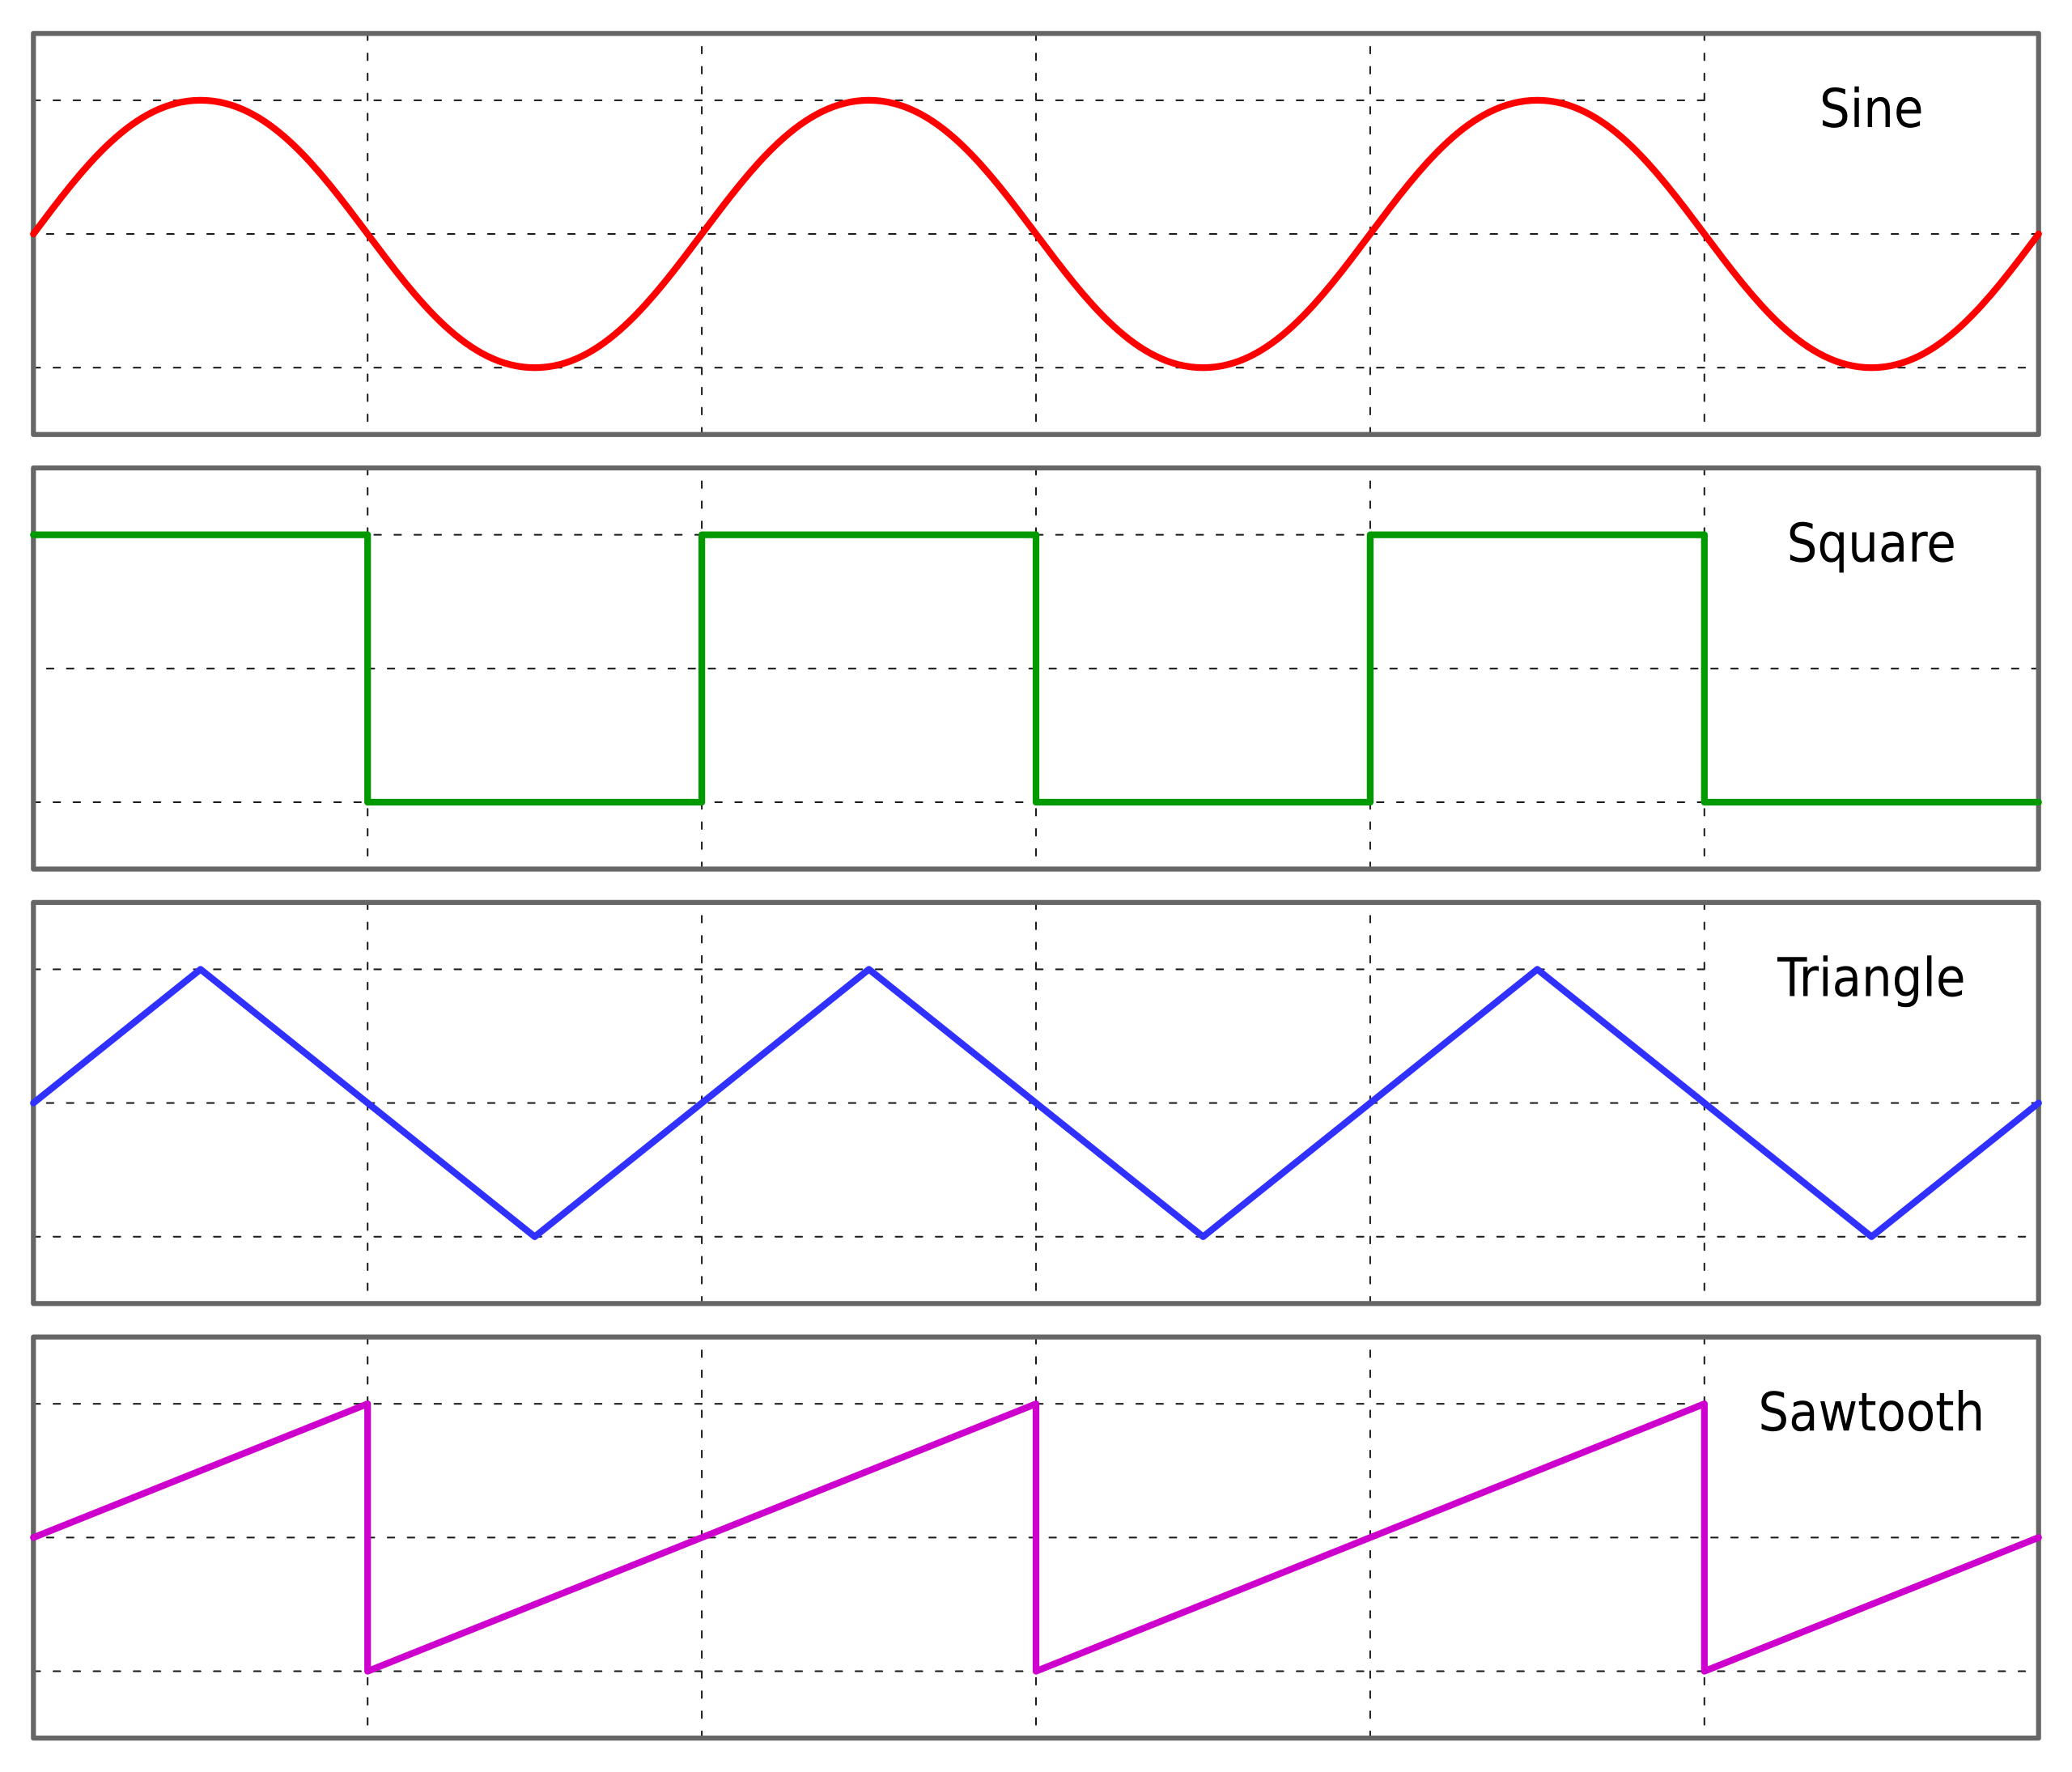
\includegraphics[width=.7\textwidth]{assets/osi/physical/waves.png}
    \caption{Theoretical waves}\label{fig:theoretical_waves}
\end{figure}

In practice, we use analog signals to transmit digital information. They are continuous and can take any value within a range. At the receiver, we need to convert them back to discrete digital values (\texttt{1} or \texttt{0}) through a process called \textbf{sampling and quantization}. The receiver samples the analog signal at specific time intervals and uses threshold levels to determine whether each sample represents a \texttt{1} or \texttt{0}.

Let's look at a simple example of a 1-bit ADC (Analog to Digital Converter) that converts a voltage level into a bit value:

% assets/osi/physical/adc_plot.png
\begin{figure}[h]
    \centering
    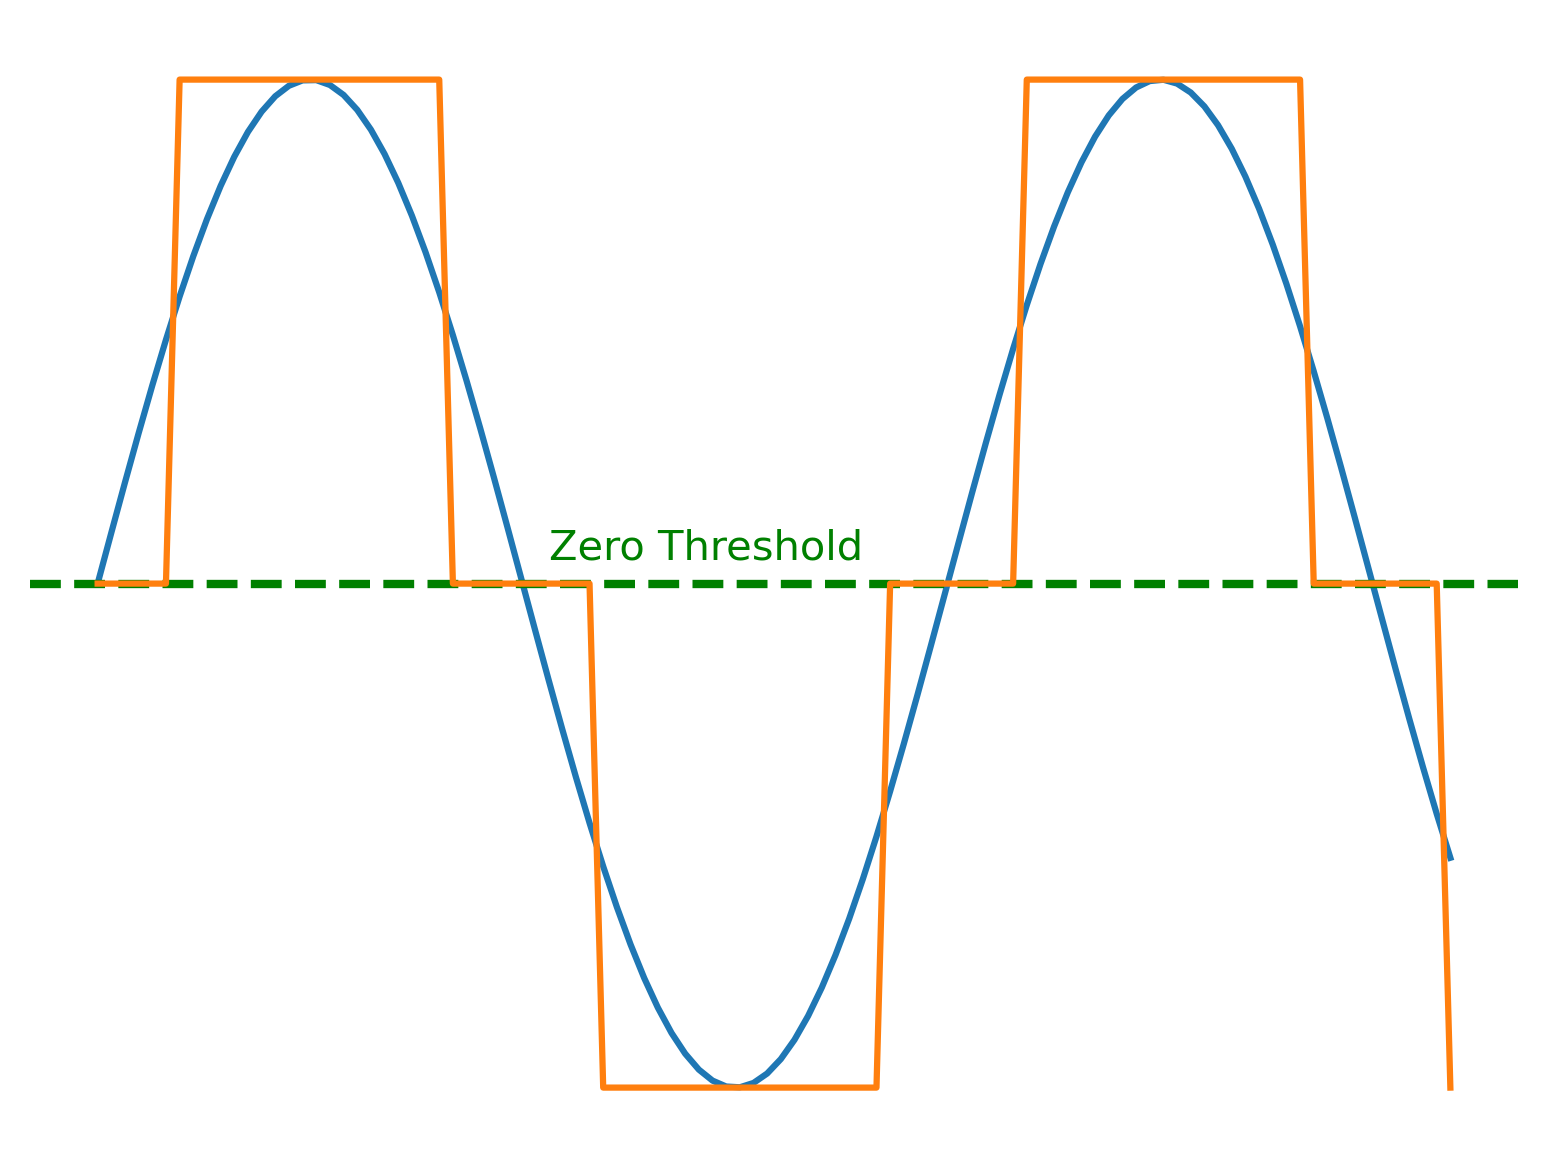
\includegraphics[width=.5\textwidth]{assets/osi/physical/adc_plot.png}
    \caption{Example of a 1-bit ADC converting voltage levels to bits}\label{fig:adc_plot}
\end{figure}

However, as you can probably guess, there are infinite ways for us to interpret this graph. It could correspond to \texttt{1010} or \texttt{1111000011110000} and so on. 
This is where clock signals come into play, which help us determine when to sample the signal and how to interpret it.

\subsection*{Let's talk timing $\star$}
Clocks or timing signals are present in all hardware communication. 

The idea is to ensure that both sender and receiver are synchronized in their understanding of when bits are being sent and received. 


There are two main types of synchronization:
\begin{itemize}
    \item Both sender and receiver share a common clock signal (Figure~\ref{fig:clock_sync}) - Synchronous 
    \item Sender and receiver do not share a common clock, but use start and stop bits to indicate the beginning and end of a data frame - Asynchronous
\end{itemize}

\begin{figure}[h]
    \centering
    \begin{tikzpicture}
        % Clock signal
        \draw[thick] (0,2) -- (0.5,2) -- (0.5,3) -- (1,3) -- (1,2) -- (1.5,2) -- (1.5,3) -- (2,3) -- (2,2) -- (2.5,2) -- (2.5,3) -- (3,3) -- (3,2) -- (3.5,2) -- (3.5,3) -- (4,3) -- (4,2) -- (4.5,2);
        \node at (-0.5,2.5) {Clock};
        
        % Data signal
        \draw[thick] (0,0.5) -- (1,0.5) -- (1,1.5) -- (2,1.5) -- (2,0.5) -- (3.5,0.5) -- (3.5,1.5) -- (4.5,1.5);
        \node at (-0.5,1) {Data};
        
        % Sampling points
        \foreach \x in {0.5,1.5,2.5,3.5}
            \draw[red,thick] (\x,0.2) -- (\x,1.8);
        
        % Bit values
        \node at (0.5,0) {0};
        \node at (1.5,0) {1};
        \node at (2.5,0) {0};
        \node at (3.5,0) {1};
        
        % Labels
        \node at (2.25,-0.5) {Bit sampling occurs on clock transitions};
    \end{tikzpicture}
    \caption{Example rising edge clock synchronization}\label{fig:clock_sync}
\end{figure}

\vfill
In asynchronous serial\footnote{
    Serial - \textit{one after another} - communication, data is sent one bit at a time over a single channel. This is in contrast to parallel communication. More on that in the Operating Systems course.
} communication, data is organized into discrete blocks called code words of fixed length - usually bytes or ASCII characters (\texttt{char}s are $2^8 = 256$ bits, i.e. a byte). Each code word is framed by:

\begin{figure}[h]
    \centering
    \input{assets/diagrams/physical.latex}
    \caption{Async serial frame structure}\label{fig:async_frame}
\end{figure}

This approach, specifically in the form that we refer to in the figure, is \textbf{character-oriented}.
\vfill
\section{Modulation and Encoding}\label{sec:modulation}
As mentioned earlier, modulation is the process of converting digital data into analog signals for transmission over a physical medium.

\begin{figure}[h]
    \centering
    
\includegraphics[width=\textwidth]{assets/osi/physical/signals/modulation.png}
    \caption{Modulation techniques}\label{fig:modulation_techniques}
\end{figure}

\subsection{The basics}
We'll start with something most people are familiar with, as it is used in consumer radios! The ones you listen to in your car or at home.

Amplitude Modulation (AM) and Frequency Modulation (FM) are two very common modulations used in radio broadcasting, where we are used to hearing music and news. We are used to tuning our radios to a specific frequency ($\approx$ 80-100 MHz for FM and usually way lower for AM) to listen to our favorite stations.

There's also Phase Modulation (PM), where the phase of the carrier wave is varied according to the input signal.
\begin{figure}[h]
    \centering
    \begin{tikzpicture}[scale=0.8]
        % AM Signal
        \begin{scope}[shift={(0,0)}]
            \draw[->] (0,0) -- (4.5,0) node[right] {$t$};
            \draw[->] (0,-1.5) -- (0,1.5) node[above] {$A(t)$};
            \draw[domain=0:4,samples=200,thick,blue] plot (\x,{(1+0.5*sin(2*\x r))*sin(20*\x r)});
        \end{scope}
        
        % FM Signal
        \begin{scope}[shift={(6,0)}]
            \draw[->] (0,0) -- (4.5,0) node[right] {$t$};
            \draw[->] (0,-1.5) -- (0,1.5) node[above] {$A(t)$};
            \draw[domain=0:4,samples=200,thick,red] plot (\x,{sin(20*\x r + 2*sin(2*\x r))});
        \end{scope}
        
        % PM Signal
        \begin{scope}[shift={(12,0)}]
            \draw[->] (0,0) -- (4.5,0) node[right] {$t$};
            \draw[->] (0,-1.5) -- (0,1.5) node[above] {$A(t)$};
            \draw[domain=0:4,samples=200,thick,green!50!black] plot (\x,{sin(20*\x r + 0.5*sin(2*\x r))});
        \end{scope}
    \end{tikzpicture}
    \caption{Graphical representation of \textcolor{blue}{AM}, \textcolor{red}{FM}, and \textcolor{green!50!black}{PM} signals.}\label{fig:modulation_math}
\end{figure}


But wait, we have only heard voices and music, not bits! How does that work?

The answer lies in \textbf{digital modulation}! While AM and FM were originally designed for analog voice transmission, the same radio frequencies can carry digital data using techniques like DMR, WSPR, and many, many more.
These digital protocols use discrete changes in amplitude, frequency, or phase to represent bits.

For example, in WSPR, a \texttt{1} might be represented by a short burst of a specific frequency, while a \texttt{0} might be represented by silence or a different frequency - this is called \textbf{frequency-shift keying (FSK)}.


\begin{figure}[h]
    \centering
    \begin{subfigure}[b]{0.2\textwidth}
        \centering
        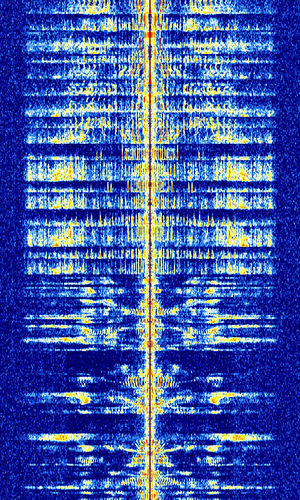
\includegraphics[width=\textwidth]{assets/osi/physical/signals/am_voice.png}
        \caption{AM Voice Signal}
        \label{fig:am_voice}
    \end{subfigure}
    \hspace{1em}
    \begin{subfigure}[b]{0.2\textwidth}
        \centering
        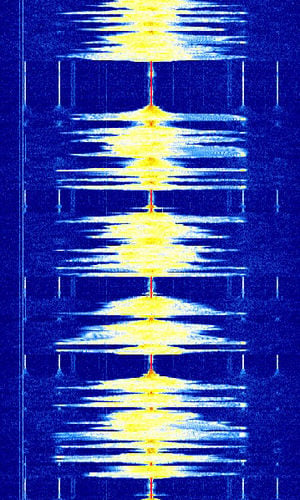
\includegraphics[width=\textwidth]{assets/osi/physical/signals/fm_voice.png}
        \caption{FM Voice Signal}
        \label{fig:fm_voice}
    \end{subfigure}
    \hspace{1em}
    \begin{subfigure}[b]{0.2\textwidth}
        \centering
        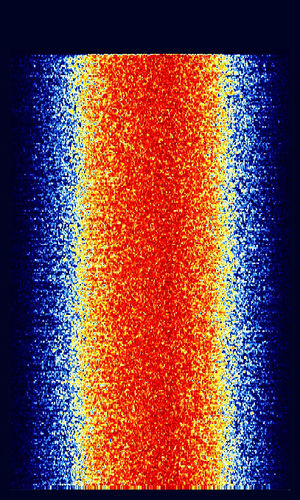
\includegraphics[width=\textwidth]{assets/osi/physical/signals/dmr.png}
        \caption{DMR Digital Signal}
        \label{fig:dmr_digital}
    \end{subfigure}
    \hspace{1em}
    \begin{subfigure}[b]{0.2\textwidth}
        \centering
        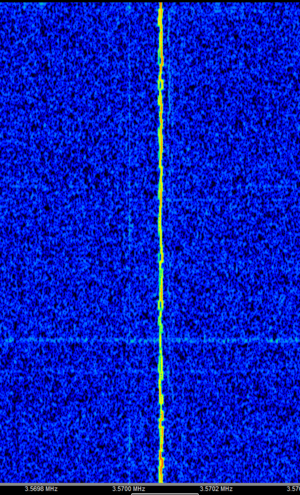
\includegraphics[width=\textwidth]{assets/osi/physical/signals/wspr.png}
        \caption{WSPR Digital Protocol}
        \label{fig:wspr_digital}
    \end{subfigure}
    
    \caption{Comparison of analog voice signals (a, b) vs digital signals (c, d) in the radio spectrum. Sourced from sigidwiki.com}
    \label{fig:analog_vs_digital_signals}
\end{figure}

\newpage
For digital data, modulation becomes synonymous with \textbf{keying}, where we use changes in the signal to represent bits.

\begin{itemize}
    \item Amplitude Shift Keying (ASK) -  A higher amplitude might represent a \texttt{1}, while a lower amplitude represents a \texttt{0}.
    \item Frequency Shift Keying (FSK) - Different frequencies represent different bits.
    \item Phase Shift Keying (PSK) - A phase shift might represent a \texttt{1}, while no shift represents a \texttt{0}.
\end{itemize}
\begin{figure}[h]
    \centering
    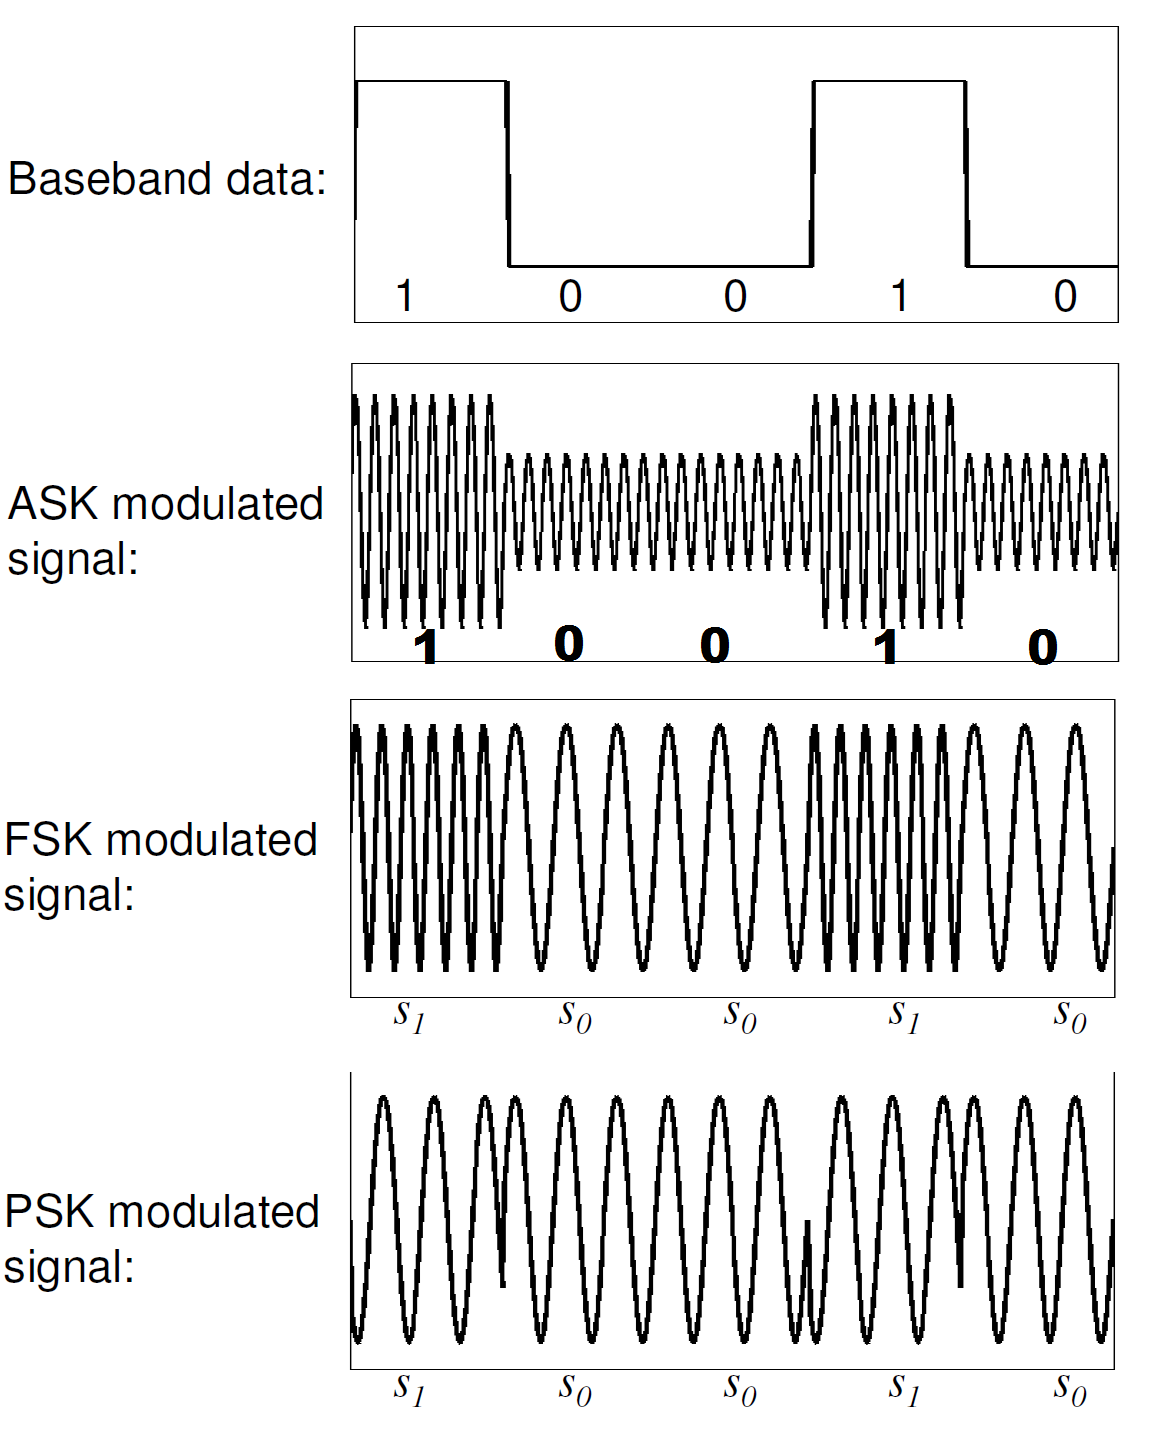
\includegraphics[width=0.45\textwidth]{assets/osi/physical/signals/sk.png}
    \caption{Keying techniques: ASK, FSK, PSK}\label{fig:keying_techniques}
\end{figure}

\subsection{Quadrature Amplitude Modulation (QAM)}
What if we could send multiple bits at once? That's where QAM comes in, which is a combination of both amplitude and phase modulation.

`Quadrature' just means we're using two waves that are perfectly out of sync - 90 degrees out of phase, to be exact (quad = four, so in a circle $\frac{360}{4} = 90$).

\subsubsection{Complex Numbers and QAM $\star$}
To completely understand QAM, we will need to quickly refresh our knowledge of complex numbers. If you are not familiar with them, I recommend reading the \href{https://en.wikipedia.org/wiki/Complex_number}{Wikipedia article}. 

QAM transmits data using two independent carrier waves at the same frequency but shifted 90 degrees apart in phase - called `in-phase' ($I$) and `quadrature' ($Q$) components. This orthogonal\footnote{
    Remember orthogonality! It's a cheat code in signal processing! It means the two signals don't interfere with each other and can be separated at the receiver.
} relationship means the two signals don't interfere with each other and can be separated at the receiver.

Complex numbers provide an elegant mathematical framework for this because:
\begin{itemize}
    \item The real part represents the in-phase ($I$) component
    \item The imaginary part represents the quadrature ($Q$) component  
    \item A 90-degree phase shift is equivalent to multiplication by $i$ (since $e^{i\pi/2} = i$)
    \item Both amplitude and phase information are present in a single complex number $z = $I$ + iQ$
\end{itemize}

\begin{figure}[h]
    \centering
    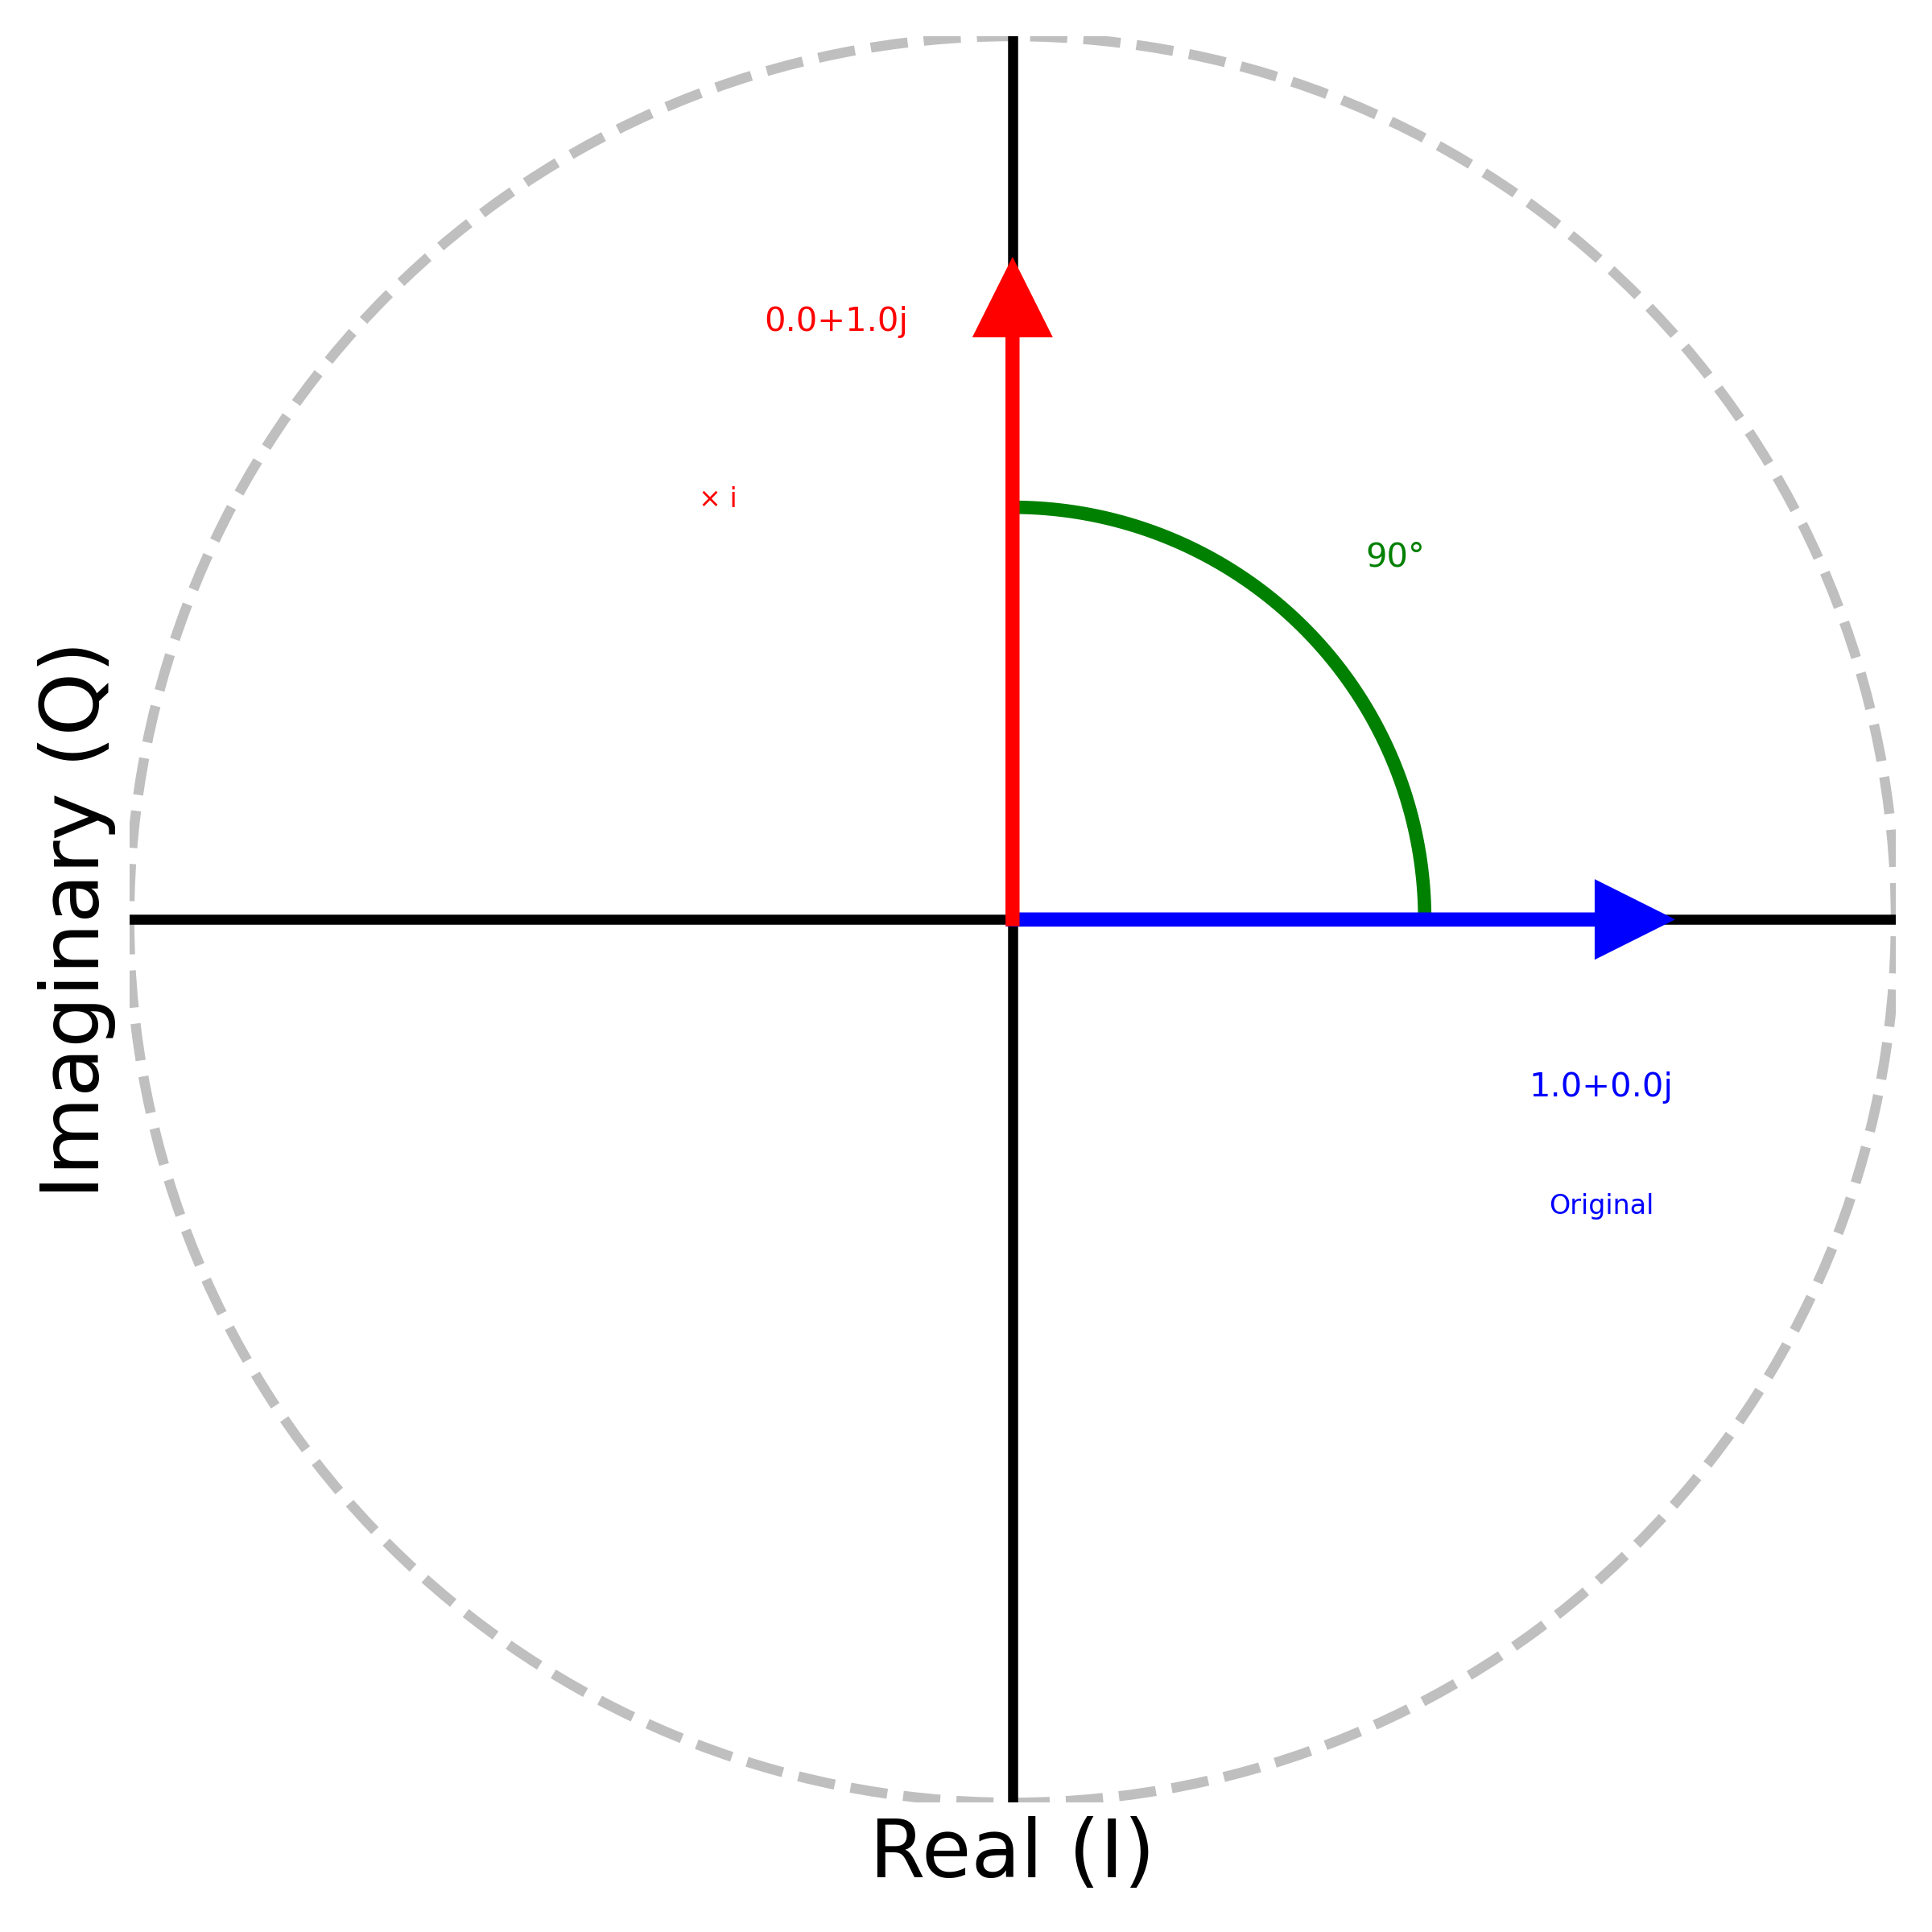
\includegraphics[width=0.5\textwidth]{assets/diagrams/iq.png}
\end{figure}

This is why we call it "Quadrature" - it literally refers to the four quadrants of this complex plane, where signals can point in any direction to encode different bit combinations.

\subsubsection{What does the number mean?}
When working with QAM, we will often see terms like 16-QAM, 64-QAM, etc. These numbers refer to the number of distinct symbols that can be transmitted. For example:
\begin{itemize}
    \item 16-QAM can transmit 16 different symbols, each representing 4 bits
    \item 64-QAM can transmit 64 different symbols, each representing 6 bits
    \item 256-QAM can transmit 256 different symbols, each representing 8 bits
\end{itemize}

You may notice the pattern in the above examples - the number of bits per symbol is given by $\log_2(N)$, where $N$ is the number of symbols.

This will immediately make sense in the next section.
\subsection{Constellation Diagrams}
A constellation diagram is a graphical representation of digital modulation schemes. Each point in the diagram represents a unique symbol that can be transmitted, with its position determined by the signal's characteristics. That's nerdspeak for points on a graph.

\begin{figure}[h]
    \centering
    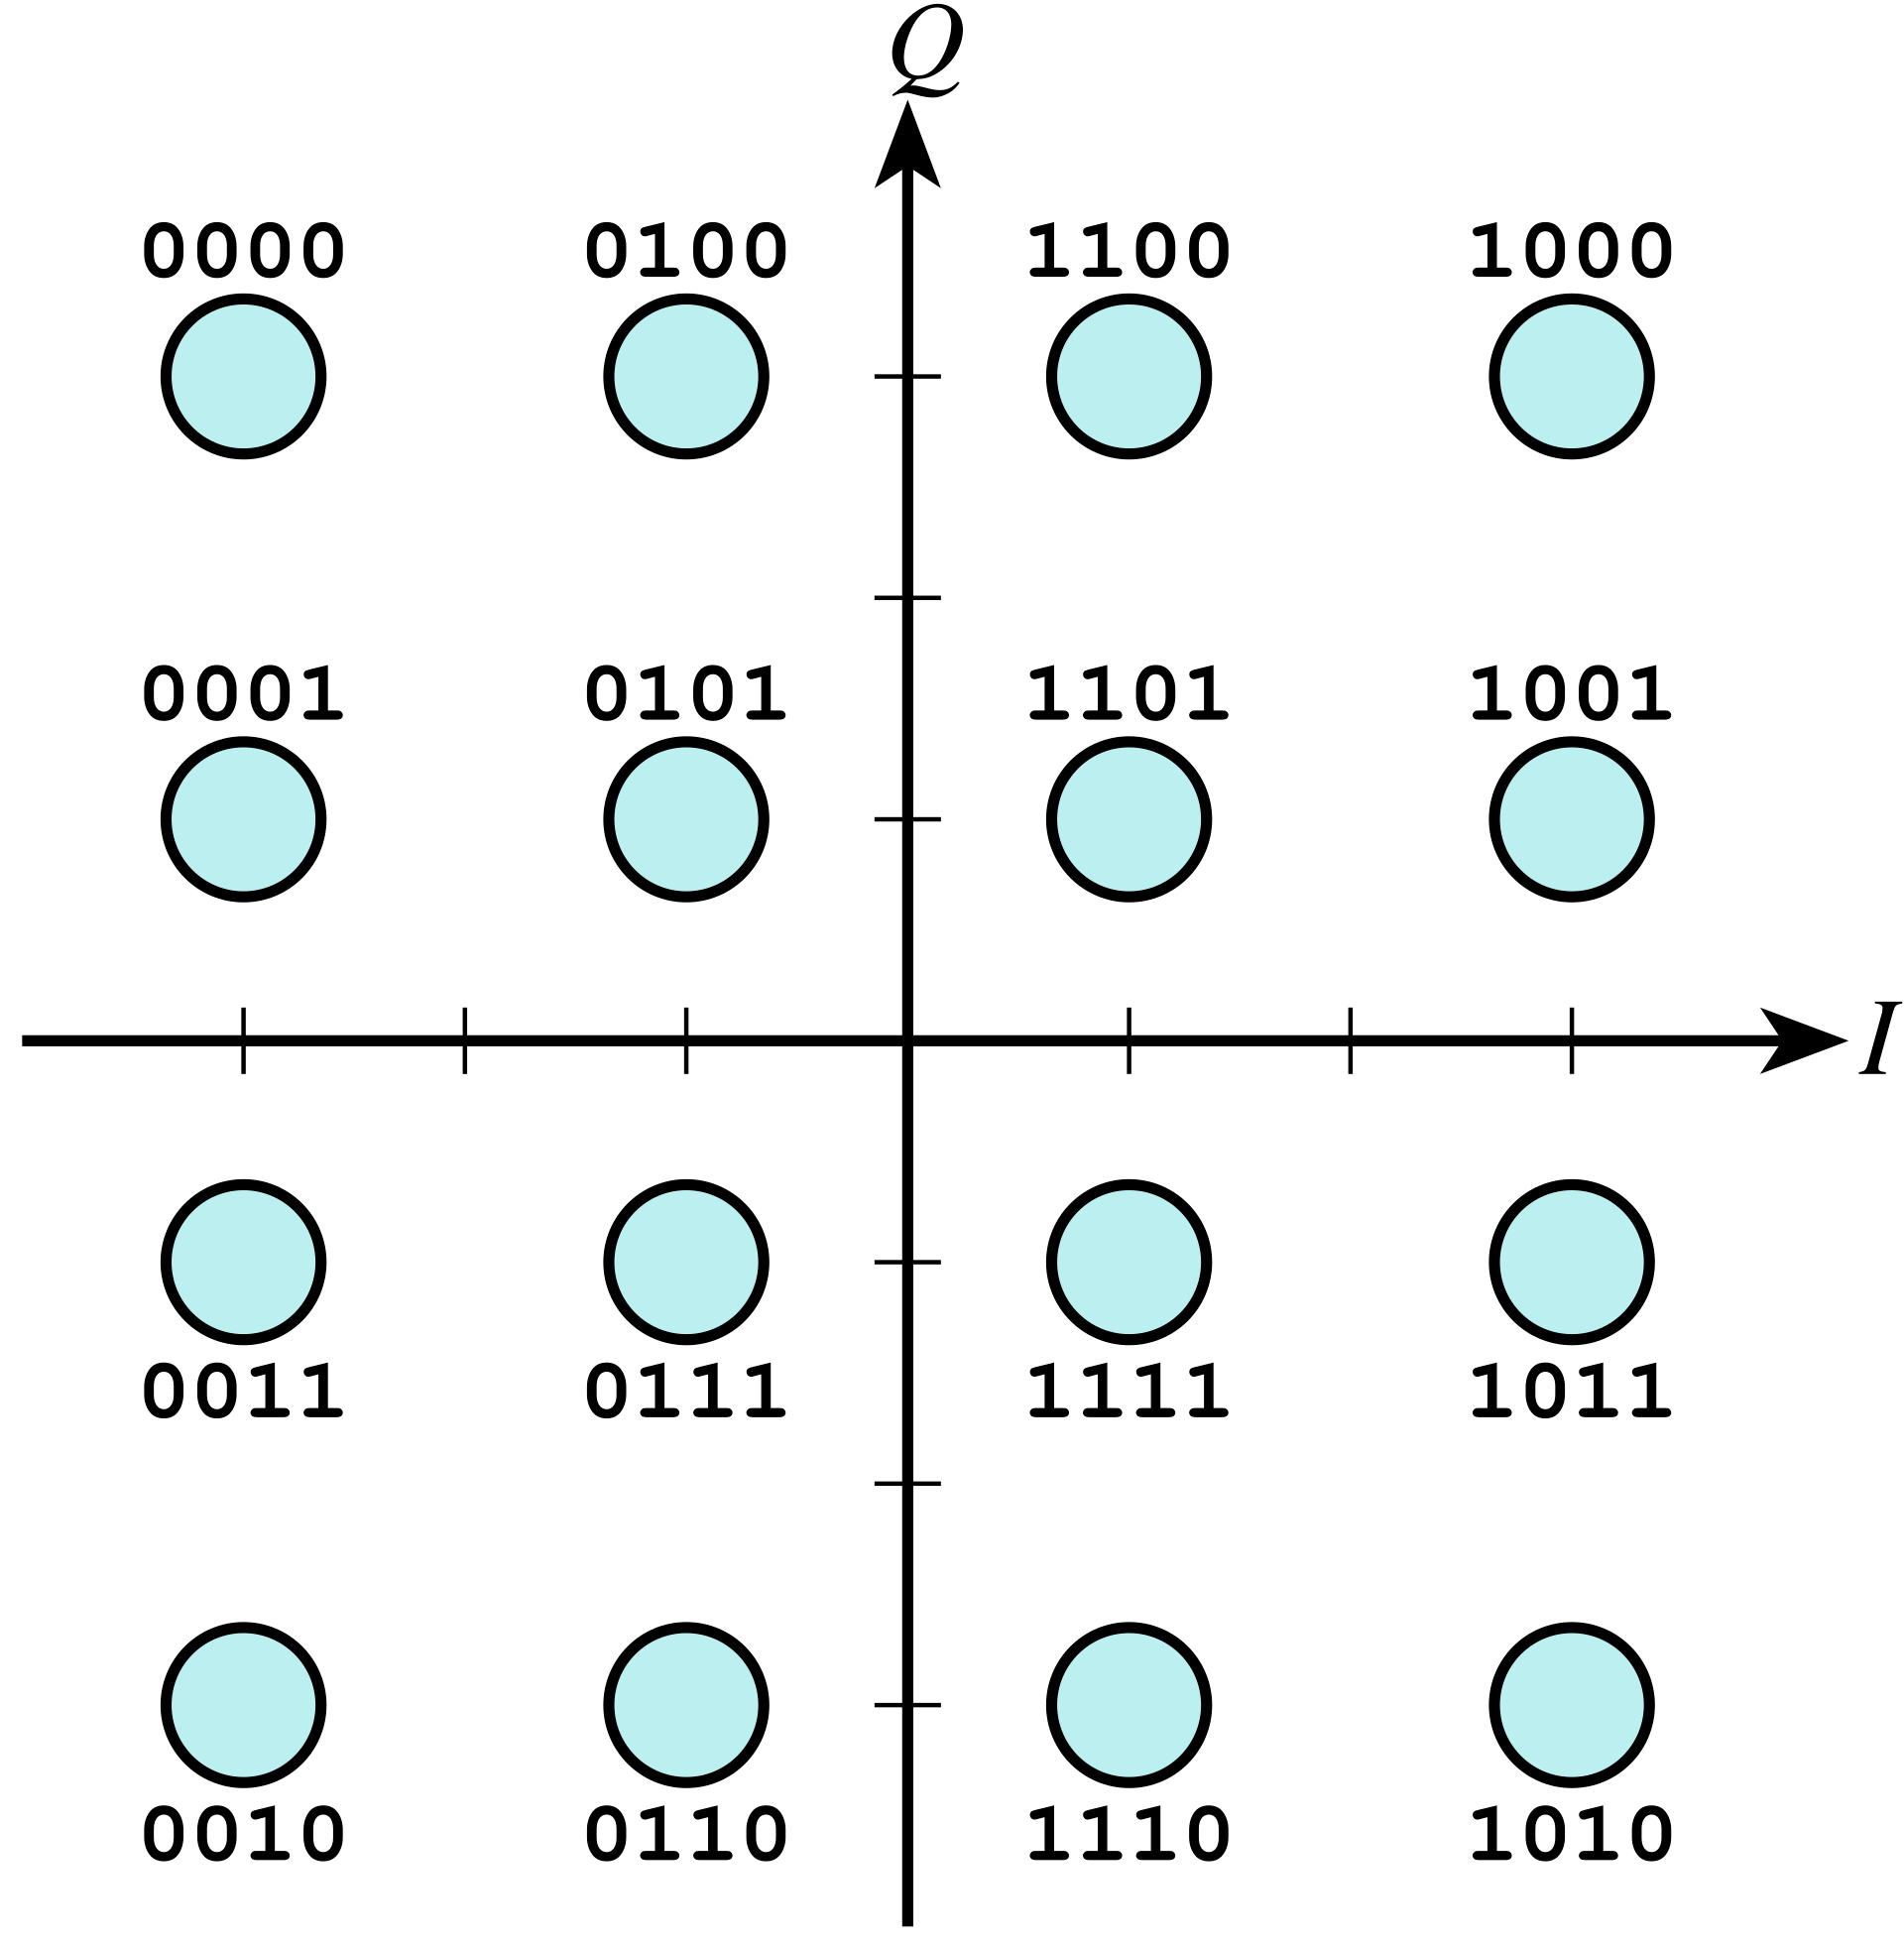
\includegraphics[width=0.5\textwidth]{assets/osi/physical/signals/qam.png}
    \caption{Example of a 16-QAM \textbf{cartesian} constellation diagram}\label{fig:qam_constellation}
\end{figure}


For QAM, the position is determined by the in-phase ($I$) and quadrature ($Q$) components (x, y coordinates). For other modulation schemes:
\begin{itemize}
    \item In PSK, points are arranged in a circle, with phase determining the angular position
    \item In ASK, points are arranged on a line, with amplitude determining the position
\end{itemize}

\begin{importantblock}
    You can probably see that ASK+PSK is QAM, since, by definition, it combines both amplitude and phase modulation.
\end{importantblock}

In any constellation diagram, each point represents a unique combination of signal parameters. The distance between points determines the minimum distance between symbols, which affects the error rate in transmission. The more points we have, the more bits we can transmit per symbol, but the closer they are together, the easier it is to confuse them at the receiver.

There are different ways to visualize these diagrams, for example, when treating ASK+PSK (component-wise, instead as a single complex number), we can plot the amplitude and phase separately as concentric circles with points scattered accross their respective circumferences. This is called a \textbf{polar constellation diagram}.

Let's look at an example of a 4-QAM (ASK+PSK) constellation diagram.
\begin{figure}[h]
    \centering
    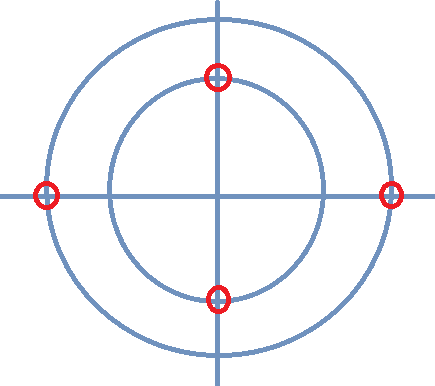
\includegraphics[width=0.5\textwidth]{assets/osi/physical/signals/ask+psk.png}
    \caption{Example of a 4-QAM \textbf{polar constellation diagram}}\label{fig:ask_psk_constellation}
\end{figure}

Now, say we want to encode the binary string \texttt{00101101}. We can map it to the 4-QAM constellation diagram as follows:

\begin{itemize}
    \item \texttt{00} maps to the first point on the left of outer circle
    \item \texttt{10} maps to the second point on the top of inner circle
    \item \texttt{11} maps to the third point on the right of outer circle
    \item \texttt{01} maps to the fourth point on the bottom of inner circle
\end{itemize}

Resulting in the following mapping:
\begin{figure}[h]
    \centering
    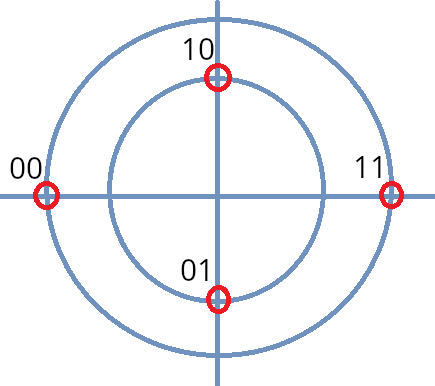
\includegraphics[width=0.5\textwidth]{assets/osi/physical/signals/ask+psk_filled.png}
    \caption{Example of a 4-QAM constellation diagram with bits mapped to points}\
    \label{fig:ask_psk_filled_constellation}
\end{figure}

Again, this mapping is arbitrary, and we can choose any mapping we want, as long as the receiver knows how to interpret it (which, hypothetically, it always does).

Since we have both amplitude and phase information for each constellation point, we can plot the actual time-domain waveforms that correspond to each symbol - showing how the signal actually looks during transmission!

Let's do so for this example.

\subsubsection{Time-Domain Waveforms}
Each constellation point can be expressed as a complex number with amplitude $A$ and phase $\phi$:
$$s(t) = A \cos(2\pi f_c t + \phi)$$

where $f_c$ is the carrier frequency. For our 4-QAM example with bit string \texttt{00101101}, the complete transmitted signal looks like:

\begin{figure}[h]
    \centering
    \begin{tikzpicture}[scale=1]
        % Main axes
        \draw[->] (0,0) -- (13,0) node[right] {Time};
        \draw[->] (0,-2) -- (0,2) node[above] {Amplitude};
        
        % Symbol boundaries (vertical dashed lines)
        \foreach \x in {3,6,9,12} {
            \draw[dashed, gray] (\x,-2) -- (\x,2);
        }
        
        % Symbol period labels
        \node[below] at (1.5,-2.3) {\texttt{00}};
        \node[below] at (4.5,-2.3) {\texttt{10}};
        \node[below] at (7.5,-2.3) {\texttt{11}};
        \node[below] at (10.5,-2.3) {\texttt{01}};
        
        % Symbol period markers
        \node[below] at (1.5,-2.6) {$T_s$};
        \node[below] at (4.5,-2.6) {$T_s$};
        \node[below] at (7.5,-2.6) {$T_s$};
        \node[below] at (10.5,-2.6) {$T_s$};
        
        % Complete waveform
        % Symbol 1: 00 (High amp, 180° phase) - inverted high amplitude cosine
        \draw[domain=0:3,samples=150,thick,blue] plot (\x,{1.5*cos(8*\x r + 180)});
        
        % Symbol 2: 10 (Low amp, 90° phase) - low amplitude sine  
        \draw[domain=3:6,samples=150,thick,red] plot (\x,{0.8*cos(8*\x r + 90)});
        
        % Symbol 3: 11 (High amp, 0° phase) - normal high amplitude cosine
        \draw[domain=6:9,samples=150,thick,green!60!black] plot (\x,{1.5*cos(8*\x r)});
        
        % Symbol 4: 01 (Low amp, 270° phase) - low amplitude negative sine
        \draw[domain=9:12,samples=150,thick,orange] plot (\x,{0.8*cos(8*\x r + 270)});
        
        % Amplitude level indicators
        \draw[dotted, gray] (0,1.5) -- (12.5,1.5) node[right] {\small High};
        \draw[dotted, gray] (0,0.8) -- (12.5,0.8) node[right] {\small Low};
        \draw[dotted, gray] (0,-0.8) -- (12.5,-0.8);
        \draw[dotted, gray] (0,-1.5) -- (12.5,-1.5);
        
        % Time axis labels
        \node[below] at (0,-0.2) {0};
        \node[below] at (3,-0.2) {$T_s$};
        \node[below] at (6,-0.2) {$2T_s$};
        \node[below] at (9,-0.2) {$3T_s$};
        \node[below] at (12,-0.2) {$4T_s$};
    \end{tikzpicture}
    \caption{Complete time-domain signal for bit string \texttt{00101101} using 4-QAM modulation. Each symbol period $T_s$ contains one constellation point with its specific amplitude and phase.}
    \label{fig:qam_complete_waveform}
\end{figure}

\begin{tipblock}
    In practice, these individual symbol waveforms are concatenated to form the complete transmitted signal. The receiver uses matched filtering and decision algorithms to determine which constellation point was transmitted by analyzing the received waveform during each symbol period.
\end{tipblock}
% multiplexing
\newpage
\section{Multiplexing}\label{sec:multiplexing}
Okay, we've covered how data gets transmitted over a medium and how we can modulate signals to represent our data. That's cool! Unfortunately, with the busy lives we lead, we need lots of data - fast! So, how do we cram all this data into our limited bandwidth? Enter multiplexing!

Multiplexing is the technique of combining multiple signals into one signal over a shared medium. This allows us to make the most out of our available bandwidth by sending multiple data streams simultaneously. It's exactly like the MUXes you've already seen in Computer Architecture, but now we're applying it to the physical layer of networking.

\subsection{Time Division Multiplexing (TDM)}
\label{subsec:tdm}
Time Division Multiplexing (TDM) shares a single link by slicing time into fixed-length slots. Each source is assigned one slot per frame; sources take turns in a periodic round-robin, so only one transmits at any instant and there is no mutual interference. If a source has nothing to send, its slot may be left idle (synchronous TDM) or reallocated on demand (statistical TDM).

\begin{figure}[h]
    \centering
    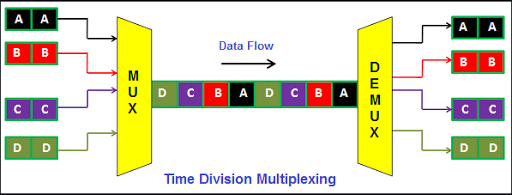
\includegraphics[width=.8\textwidth]{assets/osi/physical/multiplexing/tdm.png}
    \caption{Time Division Multiplexing (TDM) example}
    \label{fig:tdm_example}
\end{figure}

\subsection{Frequency Division Multiplexing (FDM)}
\label{subsec:fdm}
Frequency Division Multiplexing (FDM) is another technique where multiple signals are transmitted simultaneously over different frequency bands. Each signal occupies a unique frequency range, allowing them to coexist without interference. This
is commonly used in radio and television broadcasting, where different channels are assigned specific frequency bands.


TODO


\subsection{Wavelength Division Multiplexing (WDM)}
\label{subsec:wdm}

Wavelength Division Multiplexing (WDM) is a specialized form of FDM used in fiber optic communication. It allows multiple optical signals to be transmitted simultaneously over a single fiber by using different wavelengths (colors) of light. This significantly increases the capacity of the fiber, enabling high-speed data transmission over long distances.


\subsection{Multiple Access}
You might come across the term "multiple access" in networking. Especially in this course. Recall that multiplexing is about sharing a medium among multiple signals (i.e. data streams), which can be thought of as a single device (or two, in the case of communication), sending multiple signals at once towards each other.

\begin{importantblock}
    Multiple access, on the other hand, is about how \textbf{multiple devices} share a medium to communicate with each other.
\end{importantblock}

\subsection{Code Division Multiple Access (CDMA)}
\label{subsec:cdma}
Code Division Multiple Access (CDMA) allows multiple signals to share the same frequency band simultaneously. Unlike TDMA or FDMA, CDMA uses unique code sequences called "chip codes" to distinguish between different users' signals.

\paragraph{How Chip Codes Work}


Each transmitter receives a unique binary sequence (chip code) with these properties:
\begin{itemize}
    \item Much longer than data bits (typically 64-128 chips per bit)
    \item Mathematically orthogonal to other users' codes
    \item Produces strong correlation when multiplied by itself
    \item Produces near-zero correlation with different codes
\end{itemize}

When sending data, each bit is multiplied by the entire chip code. The receiver recovers the original data by multiplying the received signal with the same code and integrating over the bit period.


\begin{figure}[h]
    \centering
    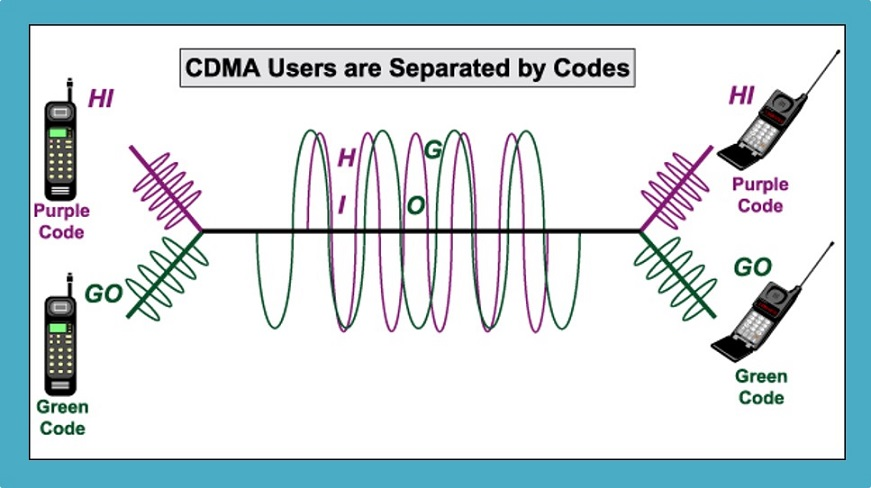
\includegraphics[width=0.7\textwidth]{assets/osi/physical/multiplexing/cdma_example.png}
    \caption{CDMA encoding showing how data bits are spread using chip codes}
    \label{fig:cdma_example}
\end{figure}


\subsubsection{Orthogonality of Chip Codes $\star$}

CDMA deals with the problem of multiple users transmitting simultaneously. We can make the analogy with multiple people talking over each other: if everyone speaks over each other, it's a mess. But if the group involved is comprise of pairs of people, each speaking their own, completely different language, they can communicate without interference (because they can't understand anyone but their partner). 

The "languages" in CDMA are called \textbf{chip codes} - patterns that are mathematically orthogonal to each other. Orthogonality, in math terms, means that two vectors are perpendicular to each other, so they don't interfere with each other when projected onto a common space.

In everyday life, orthogonality appears in many forms. Think of noise-canceling headphones: they work by generating sound waves that are "orthogonal" (phase-inverted) to ambient noise, effectively canceling it out. Similarly, polarized sunglasses use orthogonal light wave orientations to block glare - light waves vibrating in one direction are blocked while those in the perpendicular direction pass through.

\begin{importantblock}
    Two codes are orthogonal when their dot product equals zero. This means they don't interfere with each other, allowing perfect separation at the receiver.
\end{importantblock}

Let's take a look at how this works in practice. We have two users, each with their own chip codes:
\begin{align*}
\vec{c_1} &= [1, -1, 1, -1]\\
\vec{c_2} &= [1, 1, -1, -1]
\end{align*}
And data:
\begin{align*}
d_1 &= [1, 0, 1, 0]\\
d_2 &= [0, 1, 0, 1]
\end{align*}

Verifying orthogonality of chip codes (just to drive the point home, you don't need to do this in practice):
\begin{align*}
\vec{c_1} \cdot \vec{c_2} &= (1)(1) + (-1)(1) + (1)(-1) + (-1)(-1)\\
&= 1 - 1 - 1 + 1 = 0
\end{align*}

\subsubsection{Encoding Data}


When encoding, each data bit controls the direction of the chip code vector:
\begin{itemize}
    \item For a bit value of 1: Use the original chip code
    \item For a bit value of 0: Use the inverted chip code (multiply by -1)
\end{itemize}

Because the chip codes are orthogonal to each other, the receiver can extract each user's data by projecting the combined signal onto their respective code direction, effectively filtering out other users' data.

So, for our running example, we have:

User 1:
\begin{align*}
d_1[0]=1: \underbrace{[1, -1, 1, -1]}_{\text{chip code for bit 1}}\\
d_1[1]=0: \underbrace{[-1, 1, -1, 1]}_{\text{chip code for bit 0}}\\
d_1[2]=1: \underbrace{[1, -1, 1, -1]}_{\text{chip code for bit 1}}\\
d_1[3]=0: \underbrace{[-1, 1, -1, 1]}_{\text{chip code for bit 0}}\\
\end{align*}
So for user 1, the encoded signal is:
\begin{align*}
\vec{s_1} &= [1, -1, 1, -1, -1, 1, -1, 1, 1, -1, 1, -1, -1, 1, -1, 1]
\end{align*}

For user 2, skipping the details, we get:
\begin{align*}
\vec{s_2} &= [-1, -1, 1, 1, 1, 1, -1, -1, -1, -1, 1, 1, 1, 1, -1, -1]
\end{align*}

Finally, the combined (transmitted) signal is:
\begin{align*}
\vec{s} &= \vec{s_1} + \vec{s_2} = [0, -2, 2, 0, 0, 2, 0, 0, 0, -2, 2, 0, 0, 2, 0, 0]
\end{align*}

\subsubsection{Decoding Data}
To decode, the receiver multiplies the received signal by each chip code and integrates over the bit period. In other words, we compute the dot product of the received signal with each chip code, generally like this:

\[
d_i = \frac{\vec{s} \cdot \vec{c_i}}{|\vec{c_i}|^2}
\quad\text{ or }\quad
d_i = \frac{\vec{s} \cdot \vec{c_i}}{\sum_{j=1}^{n} c_{i,j}^2}
\quad\text{ or even }\quad
d_i = \frac{\sum{s_j c_{i,j}}}{\sum_{j=1}^{n} c_{i,j}^2}
\]

Where $d_i$ is the decoded data for user $i$, $\vec{s}$ is the received signal, and $\vec{c_i}$ is the chip code for user $i$. The denominator normalizes the result based on the length of the chip code. Try to understand why this works: it essentially projects the received signal onto the chip code vector, giving us the original data bit.

In pure English, the process works as follows:
\begin{enumerate}
    \item Take the received combined signal for one bit period
    \item Project it onto each user's chip code direction (dot product)
    \item The projection magnitude tells us the bit value:
    \begin{itemize}
        \item Positive projection → bit = 1
        \item Negative projection → bit = 0
        \item Zero projection → no signal from this user
    \end{itemize}
\end{enumerate}

For user 1, decoding the first bit:
For user 1, decoding the first bit:
\begin{align*}
d_{1,0} &= \frac{\sum_{j=0}^{3} s_j c_{1,j}}{\sum_{j=0}^{3} c_{1,j}^2}\\
&= \frac{(0)(1) + (-2)(-1) + (2)(1) + (0)(-1)}{(1)^2 + (-1)^2 + (1)^2 + (-1)^2}\\
&= \frac{0 + 2 + 2 + 0}{1 + 1 + 1 + 1}\\
&= \frac{4}{4} = 1
\end{align*}

Similarly, for all bits and users:

User 1:
\begin{align*}
d_{1,0} &= \frac{\sum_{j=0}^{3} s_j c_{1,j}}{\sum_{j=0}^{3} c_{1,j}^2} = \frac{4}{4} = 1 \\
d_{1,1} &= \frac{\sum_{j=4}^{7} s_j c_{1,j}}{\sum_{j=0}^{3} c_{1,j}^2} = \frac{-4}{4} = -1 \approx 0 \\
d_{1,2} &= \frac{\sum_{j=8}^{11} s_j c_{1,j}}{\sum_{j=0}^{3} c_{1,j}^2} = \frac{4}{4} = 1 \\
d_{1,3} &= \frac{\sum_{j=12}^{15} s_j c_{1,j}}{\sum_{j=0}^{3} c_{1,j}^2} = \frac{-4}{4} = -1 \approx 0
\end{align*}

User 2:
\begin{align*}
d_{2,0} &= \frac{\sum_{j=0}^{3} s_j c_{2,j}}{\sum_{j=0}^{3} c_{2,j}^2} = \frac{-4}{4} = -1 \approx 0 \\
d_{2,1} &= \frac{\sum_{j=4}^{7} s_j c_{2,j}}{\sum_{j=0}^{3} c_{2,j}^2} = \frac{4}{4} = 1 \\
d_{2,2} &= \frac{\sum_{j=8}^{11} s_j c_{2,j}}{\sum_{j=0}^{3} c_{2,j}^2} = \frac{-4}{4} = -1 \approx 0 \\
d_{2,3} &= \frac{\sum_{j=12}^{15} s_j c_{2,j}}{\sum_{j=0}^{3} c_{2,j}^2} = \frac{4}{4} = 1
\end{align*}

So we've successfully recovered our original data: $d_1 = [1, 0, 1, 0]$ and $d_2 = [0, 1, 0, 1]$.

\newpage
\subsection{TDMA and FDMA}
\label{subsec:tdma_fdma}

Now that we've seen how CDMA works, let's look at two other fundamental multiple access techniques: TDMA and FDMA. These approaches solve the same problem (multiple users sharing a medium) but use completely different strategies.

\subsubsection{TDMA}
Think of TDMA like a well-organized conversation. Everyone gets to speak, but they take turns - only one person talks at a time, and everyone else listens. When your turn comes, you have the floor completely to yourself.

This approach to resource allocation is called \textbf{round-robin} schedule: users take turns in a fixed order, each occupying one time slot per frame; after the last user, the sequence repeats.

\begin{figure}[h]
    \centering
    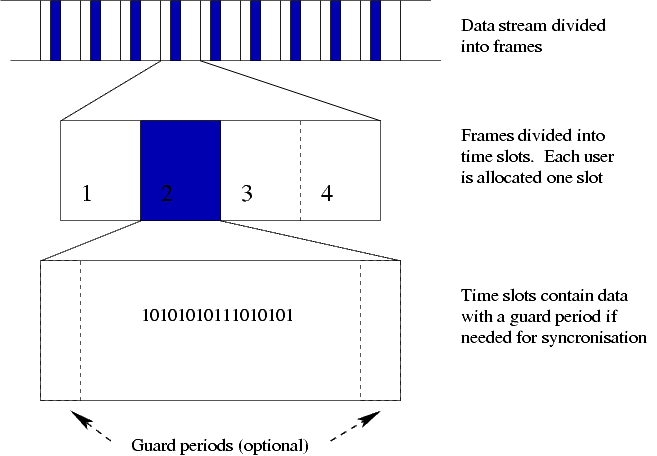
\includegraphics[width=0.8\textwidth]{assets/osi/physical/multiplexing/tdma.png}
    \caption{TDMA: Users take turns transmitting in fixed time slots}
    \label{fig:tdma}
\end{figure}

In TDMA:
\begin{itemize}
    \item The entire frequency band is available to each user
    \item Time is divided into fixed slots (called a "frame")
    \item Each user gets one slot per frame
    \item Users transmit in round-robin fashion
    \item If a user has nothing to send, their slot remains empty
\end{itemize}


\subsubsection{FDMA}
FDMA has multiple dedicated perceptual "lanes" that users can occupy called channels. This is like FM radio, WiFi or even cable TV, where each channel is a separate frequency band.

\begin{figure}[h]
    \centering
    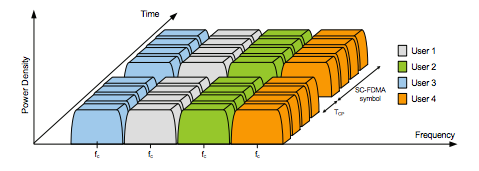
\includegraphics[width=0.8\textwidth]{assets/osi/physical/multiplexing/fdma-sc.png}
    \caption{FDMA: Users transmit simultaneously on different frequency bands}
    \label{fig:fdma}
\end{figure}

In FDMA:
\begin{itemize}
    \item Each user gets a dedicated frequency band (channel)
    \item All users can transmit simultaneously
    \item Guard bands separate channels to prevent interference
    \item Users can transmit whenever they want within their assigned frequency
\end{itemize}

Modern systems often combine these techniques! For example:
\begin{itemize}
    \item \textbf{4G LTE}: Uses both FDMA (different frequency carriers) and TDMA (time slots within each carrier)
    \item \textbf{Wi-Fi}: Uses FDMA (different channels) plus collision avoidance protocols
    \item \textbf{GPS}: Uses CDMA for satellites plus FDMA for different frequency bands
\end{itemize}

\begin{importantblock}
    Remember: These are all solutions to the same fundamental problem - how do multiple users share a limited communication medium without interfering with each other? The "best" solution depends on your specific requirements for capacity, latency, complexity, and cost.
\end{importantblock}

\subsection{Carriers and Sensing}
\label{subsec:carriers_sensing}
As you might have noticed in Figure \ref{fig:fdma}, the graph is labelled as FDMA-SC, where the SC stands for \textbf{Single Carrier}. But what is a carrier? We've also seen that word in Section \ref{sec:modulation} when we talked about modulating signals.

\begin{importantblock}
    A carrier is a signal that can be modulated to carry information. Usually a sine wave, we augment it by modulating its amplitude, frequency, or phase to encode our data (as we mentioned in Section \ref{sec:modulation}).
\end{importantblock}

Sensing is the process of detecting whether a signal is already present on a carrier frequency. This allows devices to determine if a channel is busy or available before attempting to transmit. In TDMA systems, sensing helps verify if it's the designated time slot for transmission. In FDMA systems, sensing checks whether the assigned frequency band is clear of interference.

This brings us to a perfect (in the author's opinion) segue: carrier sensing addresses collision detection, but collision handling and recovery falls under the Data Link Layer of the OSI model. You're in luck! Enter\dots



% Datalink Layer
\chapter{Data Link Layer}\label{sec:datalink_intro}
Well! We've finally made it past the Physical Layer, which is a good thing, because it can be pretty boring. The Data Link Layer is where things start to get interesting, as it is the first layer that deals with actual data packets and their transmission over a physical medium.


\section{What is the Data Link Layer?}
The Data Link Layer is the second layer of the OSI model, sitting above the Physical Layer and below the Network Layer. It provides node-to-node\footnote{
    directly connected devices, \textbf{not} end-to-end communication!!!
} data transfer and handles error correction from the Physical Layer. The Data Link Layer is responsible for framing, addressing, and error detection and correction.

It's further divided into two sublayers - the Logical Link Control (LLC) and the Media Access Control (MAC). The LLC sublayer is responsible for managing communication between devices, while the MAC sublayer handles access to the physical medium. 

If you were to run \texttt{ifconfig} on a Linux machine, you would see the MAC address of your network interface card (NIC) listed under each interface\footnote{
    Interfaces are the logical representations of your network connections, such as Ethernet or Wi-Fi. It is not tied to hardware, but rather to the software that manages the hardware. There exist virtual interfaces as well, which are used for things like VPNs and Docker containers.
}'s \texttt{ether} field.

\begin{verbatim}
$ ifconfig
wlan0: flags=4163<UP,BROADCAST,RUNNING,MULTICAST>  mtu 1500
    inet 10.0.0.100  netmask 255.255.255.0  broadcast 10.0.0.255
    inet6 fe80::f00d:dead:1337:d00d  prefixlen 64  scopeid 0x20<link>
    ether f0:0d:de:ad:13:37  txqueuelen 1000  (Ethernet) <---- MAC address
    RX packets 80085  bytes 5551234 (5.5 MB)
    TX packets 31415  bytes 2718281 (2.7 MB)
\end{verbatim}


% collisions
\section{Collisions}\label{sec:collisions}
Continuing from the previous section (\ref{subsec:carriers_sensing}), we now turn our attention to one of the challenges of networking: collisions. 

A collision happens when two or more devices decide to "speak" (transmit data) at the exact same time over the same communication channel. You can imagine why that's problematic. The most common way of dealing with this is to either detect the collision and retransmit the corrupted data or to avoid the collision altogether.

Collisions come in various ca;ibers - partial corruption affects only portions of data, full destruction where entire frames are lost. A particularly interesting case is the hidden terminal problem, where two devices can't detect each other's presence but attempt to communicate with the same destination simultaneously. We'll explore this phenomenon later in the chapter.

Your network interface card (NIC) constantly manages these collision scenarios, implementing detection and recovery mechanisms to maintain reliable communication.
\vfill
% /assets/diagrams/csma/collisions.png
\begin{figure}[h]
    \centering
    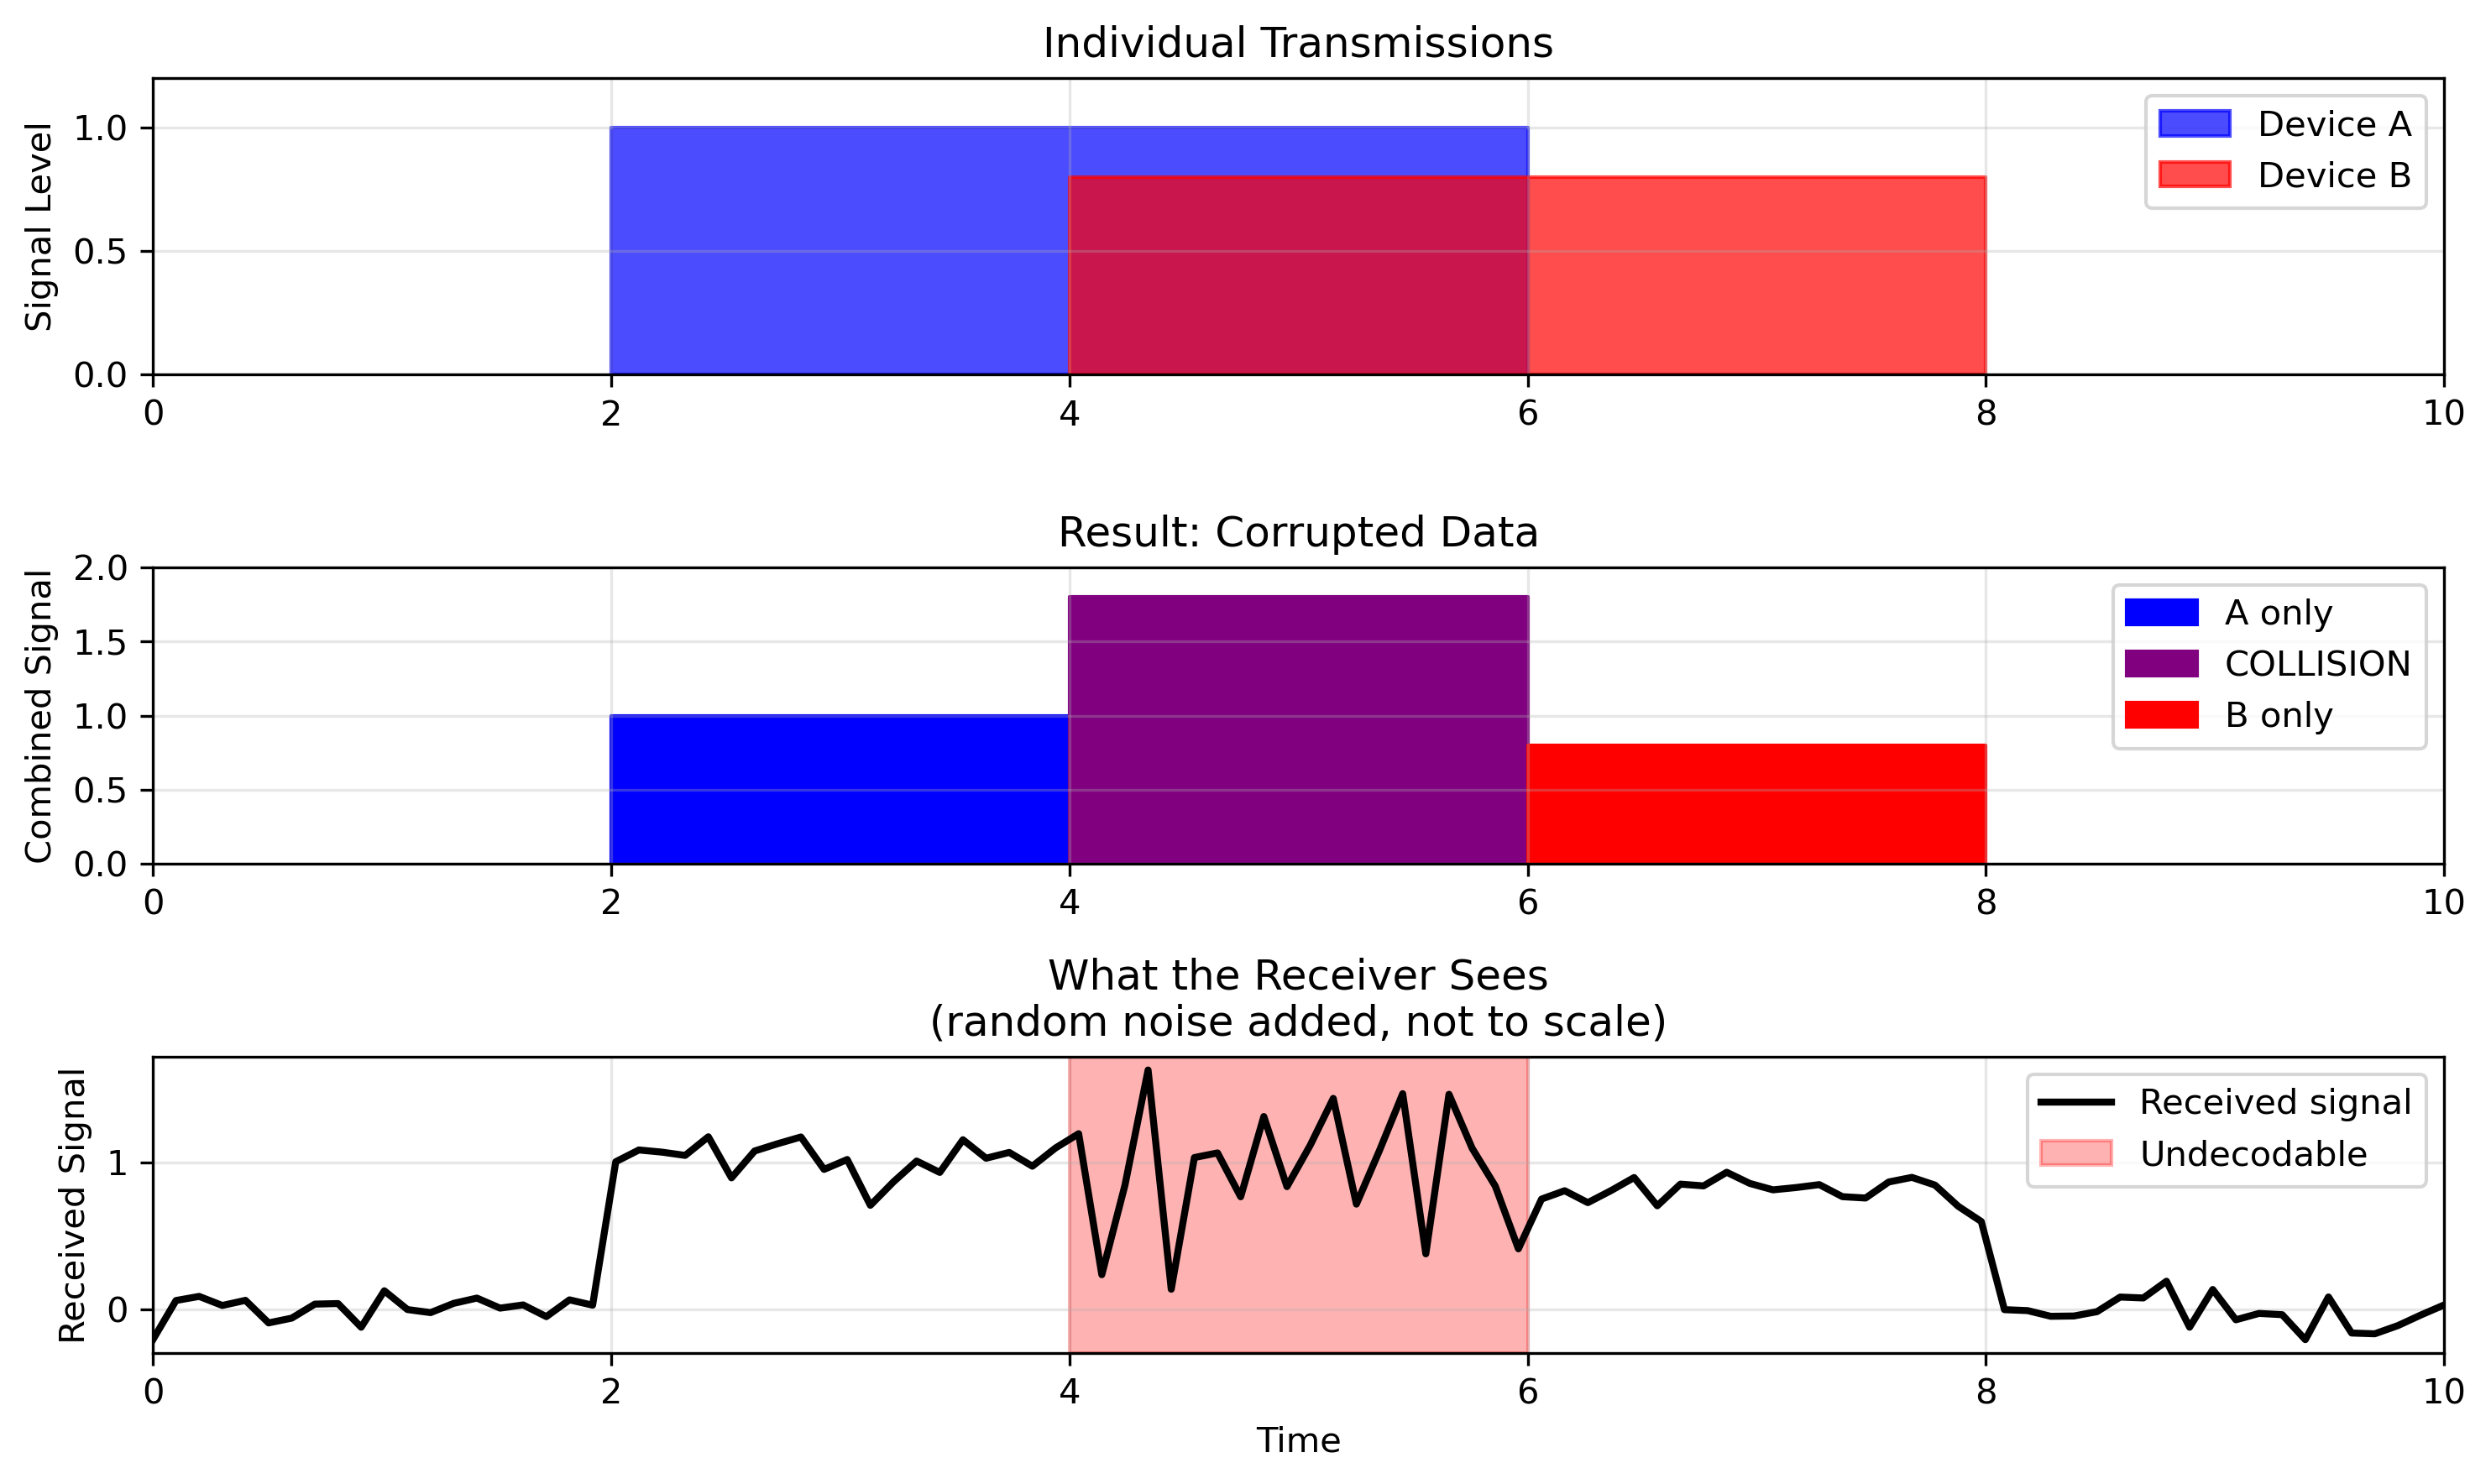
\includegraphics[width=\textwidth]{assets/diagrams/csma/collisions.png}
    \caption{Example of a collision}
    \label{fig:collision_visualization}
\end{figure}

\newpage
\subsection{Carrier Sense Multiple Access (CSMA)}
Now that we understand the problem, let's understand one of the solutions.

CSMA works on a simple principle: before transmitting anything, a device listens to the channel to see if anyone else is already talking (carrier sensing). If the channel is free, it goes ahead and transmits. If someone else is already using the channel, it waits for its turn (busy waiting).

\begin{figure}[h]
    \centering
    \scalebox{0.7}{\input{assets/diagrams/csma/normal.latex}}
    \caption{CSMA Flowchart}
    \label{fig:csma-normal}
\end{figure}

\subsubsection{+ Collision Detection (CSMA/CD)}
CSMA/CD introduces real-time collision detection. The only difference from the barebones version is that while transmitting, devices continue listening to the channel. If they detect that their signal has been corrupted by interference (collision), they immediately stop transmitting and implement a "backoff" strategy.

The backoff algorithm uses exponential backoff, meaning that after multiple failed attempts, devices wait progressively longer before retrying. This prevents starvation\footnote{
    Starvation is a scheduling problem where a process is perpetually denied the resources it needs to proceed, often due to other processes monopolizing those resources or the algorithm causeing it to wait indefinitely.
}.
\subsubsection{+ Collision Avoidance (CSMA/CA)}
As the name implies, CSMA/CA tries to avoid colissions entirely.

The protocol uses a handshake mechanism called RTS/CTS (Request to Send/Clear to Send).

\speechleft{Device A}{"May I please transmit to Device C?" (RTS)}
\speechright{Device C}{"Yes, go ahead, I'm ready to listen" (CTS)}
\begin{tcolorbox}[colback=gray!10, colframe=gray!50, arc=3mm, left=2mm, right=2mm, boxrule=1pt, before skip=5mm, after skip=5mm]
    \textit{Other devices hear this exchange and know to stay quiet during the upcoming transmission}
\end{tcolorbox}
\speechleft{Device A}{\textit{Transmits data with confidence}}

You'll notice how prevalent this type of conversation (protocol design) is in networking. ACKs and NACKs and handshakes are everywhere! Network people have found that this approach works well and provides much needed structure to the communication process.

\subsection{Persistence}
You might also be wondering how long a device should wait before trying to transmit again after a collision or when the channel becomes free. I guarantee you that this is something you have already thought about, but this is just about putting a name to it. 


\subsubsection{1-Persistent CSMA}
In 1-persistent CSMA, when a device finds the channel busy, it continuously monitors the channel and transmits immediately when it becomes free. This is the most aggressive approach - devices are "persistent" with probability 1.

While this minimizes delay when the channel becomes available, it also maximizes the probability of collisions when multiple devices are waiting. If two or more devices are listening to a busy channel, they will all attempt to transmit simultaneously once it's free.

\subsubsection{Non-Persistent CSMA}
Non-persistent CSMA takes the opposite approach. When a device finds the channel busy, it waits for a random amount of time before checking again, rather than continuously monitoring.

This reduces the collision probability since devices don't all rush to transmit at the exact moment the channel becomes free. However, it can lead to wasted channel capacity - the channel might sit idle while devices are in their random wait periods.

\subsubsection{p-Persistent CSMA}
p-persistent CSMA offers a compromise between the two extremes. When the channel becomes free, each device transmits with probability \textit{p}, or waits until the next time slot with probability \textit{(1-p)}.

The value of \textit{p} can be tuned based on network conditions - lower values reduce collisions but increase delay, while higher values do the opposite. This approach is commonly used in slotted networks where time is divided into discrete slots.

% /assets/osi/datalink/csma/persistence.png
\begin{figure}[h]
    \centering
    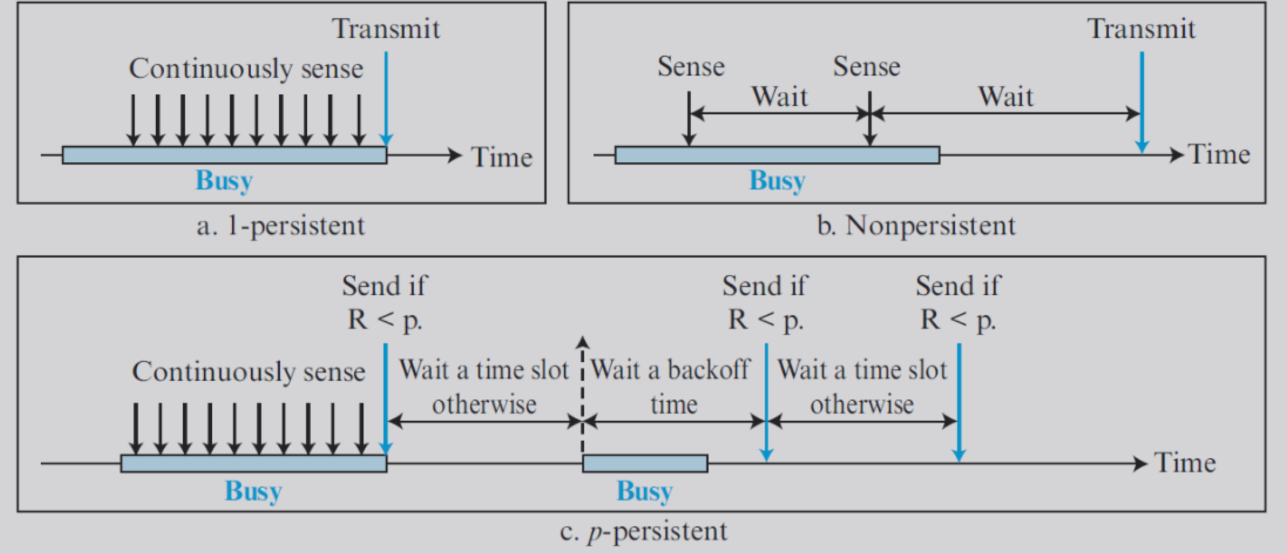
\includegraphics[width=.8\textwidth]{assets/osi/datalink/csma/persistence.png}
    \caption{Persistence in CSMA}
    \label{fig:csma-persistence}
\end{figure}
% framing
\section{Framing}\label{sec:framing}
When you need to send data over a network, you can't just throw it out there and hope for the best (unless you're UDP, which does exactly that). You need to package it up in a way that makes sense to the receiving device. This is where framing comes into play.

Framing is the process of encapsulating data into discrete units called frames. Each frame contains not only the actual data being sent but also additional information that helps the receiving device understand how to process it. This includes things like source and destination addresses, error-checking information, and control information. We'll go through some frame structure diagrams \textit{a lot} in this reader, so get used to it!

\section{Ethernet}
\label{sec:ethernet}
Ethernet is the most widely used local area network (LAN) technology today. It defines both the physical layer specifications (cables, connectors) and the data link layer framing protocol.

\subsection{Ethernet Frame Structure}
Remember when I said you should get used to frame structure diagrams? Well, here's one for Ethernet:

\begin{figure}[h]
    \centering
    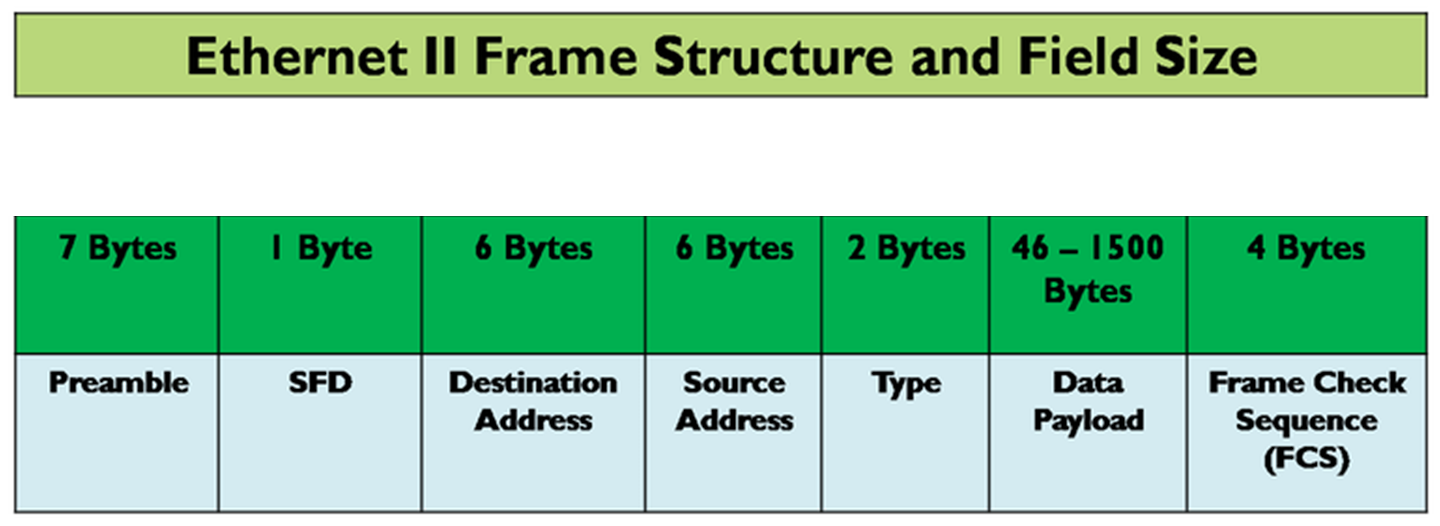
\includegraphics[width=\textwidth]{assets/osi/datalink/protocols/ethernet.png}
    \caption{Ethernet Frame Structure}
    \label{fig:ethernet_frame_structure}
\end{figure}

\begin{itemize}
\item \textbf{Preamble (7 bytes):} A sequence of alternating 1s and 0s used for synchronization
\item \textbf{Start Frame Delimiter (1 byte):} Marks the beginning of the frame with pattern 10101011
\item \textbf{Destination Address (6 bytes):} MAC address of the receiving device
\item \textbf{Source Address (6 bytes):} MAC address of the sending device
\item \textbf{Type/Length (2 bytes):} Indicates either the protocol type or frame length
\item \textbf{Data (46-1500 bytes):} The actual payload being transmitted
\item \textbf{Frame Check Sequence (4 bytes):} CRC-32 checksum for error detection
\end{itemize}


Different Ethernet standards may have variations in frame size and structure, but the basic components remain consistent. The minimum frame size is 64 bytes, and the maximum is 1518 bytes (or 1522 bytes with VLAN tagging).

\newpage
There are different physical specifications as well, which you will never need in real life, but might come across on the exam. If you need a refresher on the different types of cables, check out Section \ref{sec:transmission_media}.

\begin{table}
    \centering
    \begin{tabular}{|c|c|c|}
        \hline
        \textbf{Ethernet Standard} & \textbf{Speed} & \textbf{Cable Type} \\
        \hline
        10BASE-T & 10 Mbps & Twisted Pair (Cat 3) \\
        100BASE-TX & 100 Mbps & Twisted Pair (Cat 5) \\
        1000BASE-T & 1 Gbps & Twisted Pair (Cat 5e or higher) \\
        10GBASE-T & 10 Gbps & Twisted Pair (Cat 6a or higher) \\
        100BASE-FX & 100 Mbps & Fiber Optic \\
        1000BASE-LX & 1 Gbps & Fiber Optic \\
        10GBASE-LR & 10 Gbps & Fiber Optic \\
        \hline
    \end{tabular}
    \caption{Common Ethernet Standards}
    \label{tab:ethernet_standards}
\end{table}

\begin{tipblock}
    The naming convention for Ethernet standards follows a pattern: \textbf{Speed + BASE + Medium}. For example, 100BASE-TX means 100 Mbps speed, baseband transmission, and twisted pair cable (T) with specific characteristics (X). The "BASE" indicates baseband\footnote{
        Baseband - entire medium is used for one signal at a time, as opposed to broadband where multiple signals can coexist. This is why Ethernet is often referred to as baseband transmission.
    } transmission (as opposed to broadband), and the suffix indicates the medium type: T for twisted pair, F for fiber, L for long-wavelength fiber.

    It's easier to remember if you think of it like this, instead of just memorizing the table.
\end{tipblock}


% error detection and correction
\section{Errors and Correction}
\label{sec:error_detection}
As mentioned in the beginning of this chapter, there are many issues that the physical layer does not concern itself with. One of those is errors in the transmission of data. The physical layer is responsible for the transmission of bits, but it does not guarantee that those bits will arrive at their destination without errors.

There are many different types of errors and approaches to mitigating/correcting them! Too many to cover in this reader, even!

\subsection{Error Handling}
Most protocols discard the frame when errors are detected. However, some wireless protocols attempt to correct the frame instead of discarding it.

\subsection{Types of Errors}
There are three primary types of errors that can occur during data transmission. \textbf{Interference} refers to unpredictable changes that can alter the shape of the signal, often caused by external factors such as electromagnetic noise or physical obstructions. 

A \textbf{single-bit error} occurs when only one bit of a given data unit has changed from its original value, typically representing the most common and least severe form of data corruption. 

In contrast, a \textbf{burst error} is more serious, involving two or more bits in the data unit that have changed, which can significantly impact data integrity and is often harder to detect and correct.

\subsection{Error Detection}
Error detection is AWESOME! But also very math heavy. The basic idea is to add some extra bits to the data being transmitted, which can be used to check if the data has been corrupted during transmission.

\subsubsection{Block Coding}
Block coding is the foundation of most error detection schemes. The concept is beautifully simple: take your original data (called the \textbf{dataword}) and systematically add extra bits (called \textbf{redundancy bits}) to create a longer \textbf{codeword}.

\begin{figure}[h]
    \centering
    \begin{tikzpicture}[scale=1.2]
        % Dataword
        \draw[thick, blue] (0,1) rectangle (3,2);
        \node at (1.5,1.5) {\textbf{Dataword}};
        \node[blue] at (1.5,0.7) {$k$ bits};
        
        % Arrow
        \draw[->, thick] (3.5,1.5) -- (4.5,1.5);
        \node at (4,2.2) {\small Redundancy};
        
        % Codeword
        \draw[thick, blue] (5,1) rectangle (8,2);
        \draw[thick, red] (8,1) rectangle (9.5,2);
        \node at (6.5,1.5) {\textbf{Data}};
        \node at (8.75,1.5) {\textbf{Check}};
        \node[blue] at (6.5,0.7) {$k$ bits};
        \node[red] at (8.75,0.7) {$r$ bits};
        \node at (7.25,0.3) {\textbf{Codeword: $n = k + r$ bits}};
    \end{tikzpicture}
    \caption{Block coding adds redundancy bits to create error-detectable codewords}
    \label{fig:block_coding}
\end{figure}

Not all possible $n$-bit patterns are valid codewords - only specific combinations are allowed. When errors occur during transmission, the received pattern might not match any valid codeword, alerting us to corruption.

\subsubsection{Parity Bits: The Simplest Error Detection}
Parity\footnote{A number's parity is the property of being even or odd. In the context of error detection, it refers to the number of 1s in a binary representation.} checking is the most basic form of error detection. We add a single bit that makes the total number of 1s in the codeword either even (\textbf{even parity}) or odd (\textbf{odd parity}).

Let's see how even parity works with a 4-bit dataword:

\begin{table}[h]
\centering
\begin{tabular}{|c|c|c|c|c|c|}
\hline
\multicolumn{4}{|c|}{Dataword} & Parity & \multicolumn{1}{c|}{Total 1s} \\
\hline
$d_3$ & $d_2$ & $d_1$ & $d_0$ & $p$ & Count \\
\hline
0 & 0 & 0 & 0 & 0 & 0 (even) \\
0 & 0 & 0 & 1 & 1 & 2 (even) \\
0 & 0 & 1 & 0 & 1 & 2 (even) \\
0 & 0 & 1 & 1 & 0 & 2 (even) \\
0 & 1 & 0 & 0 & 1 & 2 (even) \\
\ldots & \ldots & \ldots & \ldots & \ldots & \ldots \\
\hline
\end{tabular}
\caption{Even parity ensures the total number of 1s is always even}
\label{tab:parity_example}
\end{table}

\textbf{Detection process:}
\begin{enumerate}
    \item Sender calculates parity bit and transmits dataword + parity
    \item Receiver counts all 1s in the received codeword
    \item If count is odd (for even parity), an error is detected
    \item If count is even, assume no error (though this isn't guaranteed!)
\end{enumerate}

\paragraph{Limitations of Simple Parity}
Simple parity can detect any \textbf{odd number} of bit errors (1, 3, 5, \ldots) but cannot detect \textbf{even numbers} of errors (2, 4, 6, \ldots). For example:

\begin{align*}
\text{Original:} \quad &1011\mathbf{0} \quad \text{(even parity, 3 ones total)}\\
\text{2-bit error:} \quad &1\mathbf{1}\mathbf{0}1\mathbf{0} \quad \text{(still even parity, 3 ones total)}
\end{align*}

The receiver would not detect this corruption! Simple parity operates on the principle of counting 1s, and when an even number of bits flip, the parity remains unchanged. In our example, the original codeword 10110 has three 1s (odd count), so with even parity we add a 0 to make it 101100 (four 1s total - even). After the 2-bit error occurs, 111100 still has four 1s (even count), so the parity check passes despite the data being corrupted.

This fundamental limitation occurs because parity checking uses modulo-2 arithmetic (XOR operations). When we flip an even number of bits, the XOR result remains the same:
\[
\text{bit}_1 \oplus \text{bit}_2 \oplus \ldots \oplus \text{bit}_n = \text{same result if even number of bits change}
\]

In fact, simple parity has a \textbf{50\% probability} of missing errors when multiple bits are corrupted - not much better than random guessing for multi-bit errors!

\paragraph{Two-Dimensional Parity}
To improve error detection, we can arrange data in a rectangular grid and add parity bits for both rows and columns:

\begin{figure}[h]
    \centering
    \begin{tikzpicture}[scale=0.8]
        % Data grid
        \foreach \i in {0,1,2} {
            \foreach \j in {0,1,2,3} {
                \draw (\j,\i) rectangle (\j+1,\i+1);
                \node at (\j+0.5,\i+0.5) {$d_{\i\j}$};
            }
        }
        
        % Row parity
        \foreach \i in {0,1,2} {
            \draw[red, thick] (4,\i) rectangle (5,\i+1);
            \node[red] at (4.5,\i+0.5) {$p_r\i$};
        }
        
        % Column parity
        \foreach \j in {0,1,2,3} {
            \draw[blue, thick] (\j,3) rectangle (\j+1,4);
            \node[blue] at (\j+0.5,3.5) {$p_c\j$};
        }
        
        \draw[purple, thick] (4,3) rectangle (5,4);
        \node[purple] at (4.5,3.5) {$p$};
        
        % Labels
        \node at (2,-0.5) {Data bits};
        \node[red] at (4.5,-0.5) {Row parity};
        \node[blue] at (2,4.5) {Column parity};
        \node[purple] at (6,4.5) {Overall parity};
    \end{tikzpicture}
    \caption{Two-dimensional parity can detect and sometimes correct single-bit errors}
    \label{fig:2d_parity}
\end{figure}

Two-dimensional parity can:
\begin{itemize}
    \item \textbf{Detect} most patterns of 2-bit and 3-bit errors
    \item \textbf{Locate and correct} single-bit errors
    \item Still fail for certain 4-bit error patterns
\end{itemize}

\subsubsection{Cyclic Redundancy Check (CRC)}
While parity bits are simple, they're not very powerful. For better error detection, we turn to Cyclic Redundancy Check (CRC) - this is actually being used in real-life networks.

CRC is based on \textbf{polynomial arithmetic} over finite fields. Don't panic! The math is elegant once you understand the pattern.

\paragraph{The Big Idea}
Think of your data as coefficients of a polynomial. For example, the bits \texttt{1101} represent:
\[
1 \cdot x^3 + 1 \cdot x^2 + 0 \cdot x^1 + 1 \cdot x^0 = x^3 + x^2 + 1
\]

CRC works by:
\begin{enumerate}
    \item Treating data as a polynomial $M(x)$
    \item Choosing a \textbf{generator polynomial} $G(x)$
    \item Computing the remainder when $x^r \cdot M(x)$ is divided by $G(x)$
    \item Appending this remainder as the CRC bits
\end{enumerate}

\begin{importantblock}
    If no errors occur, the received codeword will be perfectly divisible by $G(x)$. If division leaves a remainder, we know errors have occurred.
\end{importantblock}

\begin{noteblock}
    CRC-32 (used in Ethernet and many other protocols) has a 32-bit check sequence and can detect virtually all error patterns in practice. The probability of an undetected error is approximately $2^{-32} \approx 2.3 \times 10^{-10}$ - incredibly small!
\end{noteblock}

TODO: CRC calculation details\ldots
% flow control
\input{sections/datalink/4_flow_control.tex}
% link management
\input{sections/datalink/5_link_management.tex}
% protocols
\input{sections/datalink/6_protocols.tex}

% ===== APPENDICES =====
\appendix


% ===== BACK MATTER =====
\backmatter
\listoffigures
\listoftables
\chapter*{Contributions}\label{sec:contributions}

\subsection*{@confestim - 28/07/25}
asdfds
\url{https://github.com/confestim/CN-Reader/pull/8}

\end{document}